\documentclass[oneside,openany]{amsdtx}
\usepackage[margin=.75in]{geometry}
\usepackage{graphicx}
\usepackage{float}
\usepackage{amsmath,amssymb}
\usepackage{url}
\usepackage[dvipsnames]{xcolor}
\usepackage{multicol}
\usepackage{fancyvrb}
\usepackage[allcolors=black]{hyperref}
\usepackage{tikz}
\usepackage{booktabs}
\usepackage{bm}
\usepackage{array}
\usepackage{enumitem}
\usepackage[T1]{fontenc}
\usepackage[utf8]{inputenc}
\usepackage[french,english]{babel}
\usepackage{listingsutf8}
\usepackage{textcomp}
\usepackage{lmodern}
\usepackage{siunitx}
\usetikzlibrary{arrows.meta,calc,fit,positioning,shapes.geometric}

\definecolor{b}{HTML}{3C78D8}
\definecolor{B}{HTML}{08357E}
\definecolor{g}{HTML}{38761D}
\definecolor{r}{HTML}{7A0101}
\definecolor{o}{HTML}{FF7F0E}
\definecolor{p}{HTML}{A64D79}
\definecolor{codegreen}{HTML}{38761D}
\definecolor{codeblue}{HTML}{000076}
\definecolor{codepurple}{HTML}{7A0101}
\definecolor{phenolicA}{HTML}{A65A2E}
\definecolor{phenolicB}{HTML}{C98A5A}
\definecolor{epoxy}{HTML}{E9C46A}
\definecolor{aluminium}{HTML}{A8B0B8}
\definecolor{gas}{HTML}{E76F51}

\lstdefinestyle{mystyle}{
  backgroundcolor=\color{white},
  commentstyle=\color{codegreen},
  keywordstyle=\color{codepurple},
  numberstyle=\ttfamily\scriptsize\color{codeblue},
  stringstyle=\color{b},
  basicstyle=\ttfamily\scriptsize,
  breakatwhitespace=false,
  breaklines=true,
  captionpos=b,
  keepspaces=true,
  numbers=left,
  numbersep=5pt,
  showspaces=false,
  showstringspaces=false,
  showtabs=false,
  tabsize=4,
  texcl=false
}
\lstset{style=mystyle,inputencoding=utf8,extendedchars=true}

\newcolumntype{L}[1]{>{\raggedright\arraybackslash}p{#1}}
\newcolumntype{M}[1]{>{\centering\arraybackslash}m{#1}}
\protected\def\code#1{\texttt{\detokenize{#1}}}
\pdfstringdefDisableCommands{\def\code#1{#1}}
\providecommand{\codepath}[1]{\path{#1}}
\newcommand{\dd}{\mathop{}\!\mathrm{d}}
\newcommand{\pd}{\partial}
\newcommand{\vect}[1]{\bm{#1}}
\newcommand{\placeholder}[1]{%
  \begin{center}
  \fbox{\begin{minipage}[c][45mm][c]{0.90\textwidth}
    \centering\color{gray}\large #1
  \end{minipage}}
  \end{center}}

\sisetup{locale=FR,per-mode=symbol,range-phrase=--,range-units=single}
\setcounter{secnumdepth}{3}
\setcounter{tocdepth}{3}

\title{~\\[-2em]\sc Modélisation Thermochimique d'un Liner Phénolique\\
dans un Moteur-fusée Solide avec ANSYS Mechanical}
\author{\sc MIT Rocket Team --- M. Nichitiu --- Simulations/Propulsion Solide}
\date{\sc 23 juillet 2026}

\begin{document}
\selectlanguage{french}
\maketitle
\begin{multicols}{2}
	{\color[HTML]{FFFFFF} .}~~~~~~~~~~~~~~~~~
\includegraphics[scale=0.1]{logos/rtlogo.pdf}\\[1em]


~\vspace{3.3em}~\\[-4.6em]{\color[HTML]{FFFFFF} .}~~~~~
\includegraphics[scale=0.2]{logos/ansys}
\end{multicols}
~\\[-1em]
\setcounter{tocdepth}{2}
\tableofcontents\vfill 
\begin{center}
\begin{minipage}{1\textwidth}
\small
\textbf{Objet du document.} \it Ce rapport décrit le modèle thermique transitoire
de pyrolyse du liner phénolique, puis son extension effectivement mise en oeuvre
dans ANSYS Mechanical pour représenter le dégazage, le soufflage et une
récession discrète par suppression d'éléments. La section consacrée à la
simulation 2 présente l'architecture numérique et un premier bilan de
performance arrêté à \(t=\SI{6.15}{s}\) sur les \SI{7}{s} prévues. Ces résultats
sont provisoires tant que le calcul n'est pas terminé. Fluent et la combustion
du propergol ne font pas partie du périmètre. Les valeurs marquées
\emph{provisoires} doivent être remplacées ou validées par des mesures du
matériau effectivement fabriqué avant toute décision de dimensionnement ou de
sécurité.
\end{minipage}
\end{center}
\vfill
% ============================================================================
\section{Contexte : Moteur à Propulsion Solide et Empilement du Carter}

\subsection{Périmètre Physique}

Le moteur étudié est un moteur-fusée à propergol solide dont le carter est
modélisé par quatre tubes coaxiaux en contact : une première couche phénolique
interne, une couche mince d'époxy, une seconde couche phénolique, puis une
enveloppe d'aluminium. Le fichier de géométrie contient les corps
\code{Phenolic0}, \code{Epoxy}, \code{Phenolic1} et \code{Alu}, qui correspondent
respectivement aux sélections nommées Mechanical \code{phe0}, \code{epo},
\code{phe1} et \code{alu}. Mechanical ne maille toutefois qu'une portion
axialement tronquée de ce modèle de référence : l'empilement radial est conservé,
mais la hauteur réduite allège le maillage et permet un temps de calcul
raisonnable. Les dimensions ci-après décrivent le moteur complet; les grandeurs
extensives calculées doivent donc être remises à l'échelle avant toute
extrapolation au moteur complet.

Le propergol n'est pas présent dans la géométrie. Son action est remplacée par
une température de gaz et un coefficient de convection imposés sur la face
interne de \code{phe0}. Il faut également préciser que le perchlorate d'ammonium
(AP) est l'\emph{oxydant} d'un propergol composite et non, à lui seul, le
combustible. La composition du liant combustible, la fraction d'aluminium
éventuelle, la pression de chambre et le profil de combustion ne sont pas
documentés dans le modèle actuel. Il est donc impossible d'en déduire un flux
pariétal de premier principe : la condition chaude actuelle demeure une donnée
d'entrée à calibrer par essai moteur ou par un modèle interne séparé.

\subsection{Dimensions et Caractéristiques du Maillage}

La revue dimensionnelle a mis en évidence un facteur deux dans l'interprétation
des cotes radiales. Les valeurs d'interface 133,350 à \SI{152.400}{mm} sont des
\emph{diamètres nominaux}, et non des rayons. Le moteur corrigé est donc un
cylindre droit de longueur \(L=\SI{1.8288}{m}\), soit exactement \SI{72}{in},
avec un alésage de \SI{133.35}{mm} (\SI{5.25}{in}) et un diamètre extérieur de
\SI{152.40}{mm} (\SI{6}{in}). L'empilement radial total vaut
\SI{9.525}{mm}.

\begin{center}
\fbox{\begin{minipage}{0.92\textwidth}
\textbf{Écart entre la conception et le calcul exécuté.}
Le STEP AP214 et la base MAPDL emploient actuellement ces mêmes valeurs comme
des \emph{rayons}; MAPDL confirme notamment
\(R_\mathrm{in}=\SI{0.13335}{m}\). Les simulations 1 et 2 déjà exécutées ont
donc un alésage numérique de \SI{266.7}{mm} et un diamètre extérieur numérique
de \SI{304.8}{mm}, soit une géométrie deux fois trop grande radialement.
Les résultats existants restent ceux de cette géométrie numérique et ne doivent
pas être présentés comme des prédictions quantitatives du moteur nominal avant
correction du modèle et nouveau calcul.
\end{minipage}}
\end{center}

\begin{figure}[H]
\centering
\begin{tikzpicture}[x=0.75cm,y=0.80cm,font=\sffamily\small,>=Latex]
  \draw[fill=gas!18,draw=gas,very thick] (0,0) rectangle (2.4,2.4);
  \draw[fill=phenolicA!72,draw=phenolicA,very thick] (2.4,0) rectangle (3.7,2.4);
  \draw[fill=epoxy!75,draw=o,very thick] (3.7,0) rectangle (4.35,2.4);
  \draw[fill=phenolicB!72,draw=phenolicA,very thick] (4.35,0) rectangle (7.25,2.4);
  \draw[fill=aluminium!72,draw=black!55,very thick] (7.25,0) rectangle (11.35,2.4);
  \node[align=center] at (1.2,1.2) {gaz chauds\\propergol\\non maillé};
  \node[rotate=90] at (3.05,1.2) {\code{phe0}};
  \node[rotate=90] at (4.025,1.2) {époxy};
  \node at (5.80,1.2) {\code{phe1}};
  \node at (9.30,1.2) {aluminium};
  \draw[->,very thick,gas] (0.15,2.75) -- (2.20,2.75)
    node[midway,above] {flux chaud \(q''_\mathrm{in}\)};
  \draw[->,very thick,o] (11.55,1.2) -- (14.8,1.2)
    node[midway,above] {convection};
  \draw[->,very thick,r] (11.55,0.85) -- (14.8,0.85)
    node[midway,below] {rayonnement};
  \draw[<->] (2.4,-0.40) -- (3.7,-0.40) node[midway,below] {\SI{1.270}{mm}};
  \draw[<->] (3.7,-1.05) -- (4.35,-1.05) node[midway,below] {\SI{0.3175}{mm}};
  \draw[<->] (4.35,-0.40) -- (7.25,-0.40) node[midway,below] {\SI{3.175}{mm}};
  \draw[<->] (7.25,-1.05) -- (11.35,-1.05) node[midway,below] {\SI{4.7625}{mm}};
  \node[anchor=west] at (0,-2.45) {\it direction radiale : intérieur \(\longrightarrow\) extérieur};
\end{tikzpicture}
\caption{Empilement radial nominal corrigé. La largeur des couches est
schématique; les cotes indiquées sont les épaisseurs radiales.}
\label{fig:stack}
\end{figure}

\begin{table}[H]
\centering
\small
\renewcommand{\arraystretch}{1.15}
\begin{tabular}{L{0.22\textwidth}M{0.20\textwidth}M{0.20\textwidth}M{0.20\textwidth}}
\toprule
\textbf{Corps} & \textbf{Diamètre intérieur} & \textbf{Diamètre extérieur} & \textbf{Épaisseur radiale} \\
 & (mm) & (mm) & (mm) \\
\midrule
\code{phe0} & 133,350 & 135,890 & 1,2700 \\
\code{epo}  & 135,890 & 136,525 & 0,3175 \\
\code{phe1} & 136,525 & 142,875 & 3,1750 \\
\code{alu}  & 142,875 & 152,400 & 4,7625 \\
\bottomrule
\end{tabular}~\\[1em]
\caption{Dimensions nominales corrigées du moteur. Une épaisseur radiale est
la moitié de la différence entre les diamètres extérieur et intérieur.}
\label{tab:geometry}
\end{table}

Pour le moteur nominal, l'aire cylindrique chaude est
\(2\pi r_i L=\SI{0.7662}{m^2}\) et l'aire extérieure vaut
\SI{0.8756}{m^2}. Dans le modèle numérique actuellement exécuté, elles valent
respectivement \SI{1.5323}{m^2} et \SI{1.7512}{m^2}. À longueur et densité
inchangées, les masses des tubes du calcul surdimensionné sont quatre fois
celles de la géométrie nominale.

Mechanical maille une tranche centrale complète de \SI{50}{mm} suivant l'axe,
soit 2,73\,\% de la longueur nominale. Le tableau~\ref{tab:mesh-dimensions}
rassemble les dimensions et les caractéristiques vérifiées dans l'export
\code{ds.dat}, la base de redémarrage et l'état de Simulation~2. La topologie
est conservée lors de la correction géométrique, mais toutes les dimensions
radiales et tailles d'élément radiales devront être divisées par deux.

\begin{table}[H]
\centering
\small
\renewcommand{\arraystretch}{1.12}
\begin{tabular}{L{0.34\textwidth}L{0.56\textwidth}}
\toprule
\textbf{Caractéristique} & \textbf{Valeur vérifiée} \\
\midrule
Domaine maillé actuel &
Tranche de \SI{50}{mm}, circonférence complète; \(r=\SI{133.350}{mm}\) à
\SI{152.400}{mm} dans la base numérique \\
Domaine nominal corrigé &
\(r=\SI{66.675}{mm}\) à \SI{76.200}{mm}; même tranche axiale si le maillage
est régénéré sans autre modification \\
Type et organisation &
Éléments thermiques 3D \code{SOLID279}; quatre volumes coaxiaux et trois
contacts thermiques liés \\
Découpage radial \code{phe0/epo/phe1/alu} &
8 / 1 / 6 / 9 couches; tailles moyennes actuelles
\SI{0.3175}{mm} / \SI{0.6350}{mm} / \SI{1.0583}{mm} /
\SI{1.0583}{mm} \\
Tailles radiales après correction &
\SI{0.15875}{mm} / \SI{0.3175}{mm} / \SI{0.5292}{mm} /
\SI{0.5292}{mm}, à topologie identique \\
Maillage volumique exporté &
\num{482900} éléments solides et \num{2242327} nœuds \\
Base MAPDL de redémarrage &
\num{630881} éléments définis après ajout des contacts et autres éléments
auxiliaires \\
Face chaude de Simulation~2 &
\num{135900} nœuds et \num{43488} éléments surfaciques; première bande de
\code{phe0}: \num{39808} éléments \\
\bottomrule
\end{tabular}
\caption{Dimensions et principales caractéristiques du maillage numérique.}
\label{tab:mesh-dimensions}
\end{table}

\subsection{Matériaux et Interfaces}

Le corps interne \code{phe0} utilise le matériau utilisateur
\code{PHENOLIC_PYROLYSIS}; \code{phe1} utilise \code{PHENOLIC_VIRGIN}; l'époxy
et l'aluminium utilisent les matériaux génériques du projet. Les trois
interfaces concentriques sont en contact thermique lié (\emph{bonded}) et
contrôlées par le programme. Cette configuration représente une adhésion parfaite
sans décollement et sans résistance thermique de contact. Elle est cohérente
pour une première étude, mais elle ne teste ni la délamination, ni la
carbonisation de l'époxy, ni la création d'un interstice gazeux.

La masse volumique initiale employée est \SI{1250}{kg.m^{-3}} pour le phénolique
vierge, \SI{1150}{kg.m^{-3}} pour l'époxy et \SI{2700}{kg.m^{-3}} pour
l'aluminium. L'alliage d'aluminium et le grade exact de l'époxy ne sont pas
spécifiés. Les propriétés associées sont donc des approximations génériques,
pas une fiche matériau qualifiée.

% ============================================================================
\clearpage
\section{Simulation 1 : Pyrolyse Volumique de la Première Couche Phénolique}

\subsection{Théorie et Dérivation}

\subsubsection{Conservation Locale de l'Énergie}

Considérons un volume matériel fixe \(V\) de phénolique, de frontière
\(\partial V\), sans mouvement macroscopique du solide. Le premier principe de
la thermodynamique impose que le taux de variation de l'énergie interne soit
égal à la puissance thermique reçue par conduction et à la production
volumique :
\begin{equation}
  \frac{\dd}{\dd t}\int_V \rho u\,\dd V
  =-\int_{\partial V}\vect q\cdot\vect n\,\dd S
   +\int_V \rho\dot q_m\,\dd V .
  \label{eq:first-law-integral}
\end{equation}
Ici \(u\) est l'énergie interne massique, \(\rho\) la masse volumique du
milieu condensé, \(\dot q_m\) une source massique et \(\vect q\) le flux de
chaleur. Le théorème de Gauss transforme le flux surfacique; comme le volume est
arbitraire,
\begin{equation}
  \frac{\pd(\rho u)}{\pd t}=-\vect\nabla\cdot\vect q+\rho\dot q_m .
\end{equation}
Avec la loi de Fourier \(\vect q=-k\vect\nabla T\), et en assimilant
\(\pd u/\pd T\) à \(c_p\) dans la formulation thermique de Mechanical, on
obtient la forme employée par le modèle :
\begin{equation}
  \rho c_p\frac{\pd T}{\pd t}
  =\vect\nabla\cdot\left(k\vect\nabla T\right)+\rho\dot q_m .
  \label{eq:heat-general}
\end{equation}

La pyrolyse est endothermique. Si \(\Delta H_p>0\) est l'enthalpie absorbée par
kilogramme de matière convertie et \(\alpha\) le degré de conversion, la source
massique est
\begin{equation}
  \dot q_m=-\Delta H_p\dot\alpha,
\end{equation}
d'où
\begin{equation}
  \boxed{\rho c_p\frac{\pd T}{\pd t}
  =\vect\nabla\cdot(k\vect\nabla T)
  -\rho\Delta H_p\dot\alpha.}
  \label{eq:heat-pyrolysis}
\end{equation}
Cette première simulation ne transporte pas l'enthalpie des gaz de pyrolyse et
ne déplace pas la frontière chaude. L'équation~\eqref{eq:heat-pyrolysis} est donc
une équation de conduction-réaction, non un modèle complet d'ablation.

\subsubsection{Variable de Conversion et Perte de Masse}

À une température donnée, on interpole entre l'état vierge \(v\) et le résidu
carbonisé \(c\). La masse volumique apparente du solide est écrite
\begin{equation}
  \rho_s(T,\alpha)=(1-\alpha)\rho_v(T)+\alpha\rho_c(T).
  \label{eq:density-mix}
\end{equation}
La définition équivalente de la conversion est
\begin{equation}
  \alpha=\frac{\rho_v-\rho_s}{\rho_v-\rho_c},\qquad 0\le\alpha\le1.
  \label{eq:alpha-density}
\end{equation}
Ainsi \(\alpha=0\) désigne la matière vierge et \(\alpha=1\) le
\emph{char} résiduel. Ce point est essentiel : \(\alpha=1\) ne signifie ni vide,
ni élément entièrement consommé. Le taux de matière volatile libérée par unité
de volume est, dans ce modèle à une réaction,
\begin{equation}
  \dot\omega'''_g=(\rho_v-\rho_c)\dot\alpha.
  \label{eq:gas-source}
\end{equation}

Les autres propriétés sont mélangées linéairement :
\begin{equation}
  X(T,\alpha)=(1-\alpha)X_v(T)+\alpha X_c(T),
  \qquad X\in\{k,c_p,\rho\}.
  \label{eq:mix-rule}
\end{equation}
Cette règle est simple et monotone, mais n'est pas une loi universelle des
composites poreux. Sa validation exige des mesures intermédiaires ou une analyse
de sensibilité.

\subsubsection{Cinétique d'Arrhenius et Intégration dans un Incrément}

La fréquence des événements moléculaires activés est représentée par une
constante d'Arrhenius
\begin{equation}
  k_r(T)=A\exp\left(-\frac{E_a}{R T}\right),
  \label{eq:arrhenius}
\end{equation}
où \(A\) est le facteur pré-exponentiel, \(E_a\) l'énergie d'activation et
\(R=\SI{8.314462618}{J.mol^{-1}.K^{-1}}\). En supposant que la quantité de sites
réactifs restante est proportionnelle à \((1-\alpha)^n\),
\begin{equation}
  \boxed{\dot\alpha=k_r(T)(1-\alpha)^n.}
  \label{eq:kinetic-law}
\end{equation}

Pendant un incrément courant \([t,t+\Delta t]\), le code prend \(T\) à la
température médiane et considère \(k_r\) constant. Posons
\(\beta=1-\alpha\). Alors \(\dot\beta=-k_r\beta^n\). Pour \(n=1\),
\begin{equation}
  \int_{\beta_0}^{\beta_1}\frac{\dd\beta}{\beta}
  =-k_r\int_t^{t+\Delta t}\dd t,
\end{equation}
donc
\begin{equation}
  \beta_1=\beta_0\exp(-k_r\Delta t),\qquad
  \boxed{\alpha_1=1-(1-\alpha_0)\exp(-k_r\Delta t).}
  \label{eq:analytic-n1}
\end{equation}
Pour \(n\ne1\), l'intégration donne
\begin{equation}
  \frac{\beta_1^{1-n}-\beta_0^{1-n}}{1-n}=-k_r\Delta t,
\end{equation}
soit
\begin{equation}
  \boxed{\beta_1=
  \left[\beta_0^{1-n}-(1-n)k_r\Delta t\right]^{1/(1-n)},
  \qquad\alpha_1=1-\beta_1.}
  \label{eq:analytic-n}
\end{equation}
Le terme entre crochets est borné pour éviter une valeur non physique. Le taux
stocké est la moyenne de l'incrément
\(\dot\alpha=(\alpha_1-\alpha_0)/\Delta t\). Le code demande une réduction du
pas si \(\Delta\alpha>0{,}05\), ce qui limite une conversion numérique trop
brutale. \emph{L'incrément courant} désigne précisément ce sous-pas accepté ou
tenté par le solveur entre deux instants convergés, et non le pas de charge
complet de sept secondes.

\subsubsection{Forme Faible à Éléments Finis}

En multipliant l'équation~\eqref{eq:heat-pyrolysis} par une fonction test
\(N_i\), puis en intégrant par parties le terme de conduction, on obtient
\begin{align}
  \int_V N_i\rho c_p\frac{\pd T}{\pd t}\,\dd V
  +\int_V \vect\nabla N_i\cdot k\vect\nabla T\,\dd V
  ={}&-\int_{\partial V}N_i\vect q\cdot\vect n\,\dd S \\
  &-\int_V N_i\rho\Delta H_p\dot\alpha\,\dd V.
  \label{eq:weak}
\end{align}
Après l'approximation \(T=\sum_jN_jT_j\), la forme matricielle est
\begin{equation}
  \vect C(T,\alpha)\dot{\vect T}
  +\vect K(T,\alpha)\vect T
  =\vect f_q-\vect f_p(T,\alpha).
\end{equation}
La dépendance de \(k\), \(c_p\), \(\rho\) et \(\dot\alpha\) à la température et
à l'historique rend le problème non linéaire. \code{UserMatTh} est appelée à
chaque point d'intégration et renvoie le flux, sa tangente, la capacité, la
densité, la source massique et les variables d'état~\cite{ansys-usermatth}.

\subsection{Configuration ANSYS Mechanical actuellement choisie}

\subsubsection{Discrétisation, contacts et conditions aux limites}

Les quatre corps utilisent des éléments thermiques volumiques \code{SOLID279}.
L'export contrôlé contient environ \num{482900} éléments solides et
\num{2242327} équations. La répartition est donnée au
tableau~\ref{tab:mesh}. Les huit couches dans \code{phe0} donnent une épaisseur
radiale moyenne de seulement \SI{0.318}{mm}, ce qui est adapté à la résolution
d'un front de pyrolyse. Même avec la troncature axiale décrite précédemment,
cette résolution radiale reste coûteuse en temps de calcul.

\begin{table}[H]
\centering
\small
\begin{tabular}{L{0.22\textwidth}M{0.18\textwidth}M{0.24\textwidth}L{0.25\textwidth}}
\toprule
\textbf{Corps} & \textbf{Éléments} & \textbf{Niveaux radiaux moyens} & \textbf{Matériau} \\
\midrule
\code{phe0} & 315536 & 8 & \code{PHENOLIC_PYROLYSIS} \\
\code{epo}  & 9516   & 1 & époxy générique \\
\code{phe1} & 59028  & 6 & \code{PHENOLIC_VIRGIN} \\
\code{alu}  & 98820  & 9 & aluminium générique \\
\bottomrule
\end{tabular}~\\[1em]
\caption{Maillage du domaine axial tronqué exporté par Mechanical.}
\label{tab:mesh}
\end{table}

Les trois paires de contact sont liées : \code{phe0_ext--epo_int},
\code{epo_ext--phe1_int} et \code{phe1_ext--alu_int}. La température initiale
est \(T_0=\SI{295.15}{K}\). La face interne reçoit
\begin{equation}
  q''_\mathrm{in}=h_\mathrm{in}(T_g-T_s),\qquad
  h_\mathrm{in}=\SI{1000}{W.m^{-2}.K^{-1}},\quad T_g=\SI{2504}{K}.
  \label{eq:inner-bc}
\end{equation}
Il s'agit de \SI{2230.85}{\degreeCelsius} dans l'interface Mechanical. À
l'extérieur, le modèle combine une convection naturelle
\(h_\mathrm{out}=\SI{8}{W.m^{-2}.K^{-1}}\) vers \SI{295.15}{K} et un
rayonnement de corps gris
\begin{equation}
  q''_\mathrm{rad}=\varepsilon\sigma(T_s^4-T_\infty^4),\qquad
  \varepsilon_\mathrm{Al}=0{,}25.
\end{equation}
Les coefficients \(h_\mathrm{in}\), \(h_\mathrm{out}\), la température des gaz et
l'émissivité sont des hypothèses du projet, non des résultats de la combustion.

L'étude est une thermique transitoire complète de \SI{7}{s}, avec pas
automatique : \(\Delta t_\mathrm{initial}=\SI{0.05}{s}\),
\(\Delta t_\mathrm{min}=\SI{0.001}{s}\),
\(\Delta t_\mathrm{max}=\SI{0.05}{s}\). La routine utilisateur ajoute son propre
critère \(\Delta\alpha\le0{,}05\). Les variables d'état sont demandées à tous
les sous-pas par \code{OUTRES,SVAR,ALL}. La configuration observée lance huit
processus DMP; la routine n'utilise aucune variable globale mutable et convient
donc aussi à un futur calcul distribué, sous réserve que la DLL soit accessible
à chaque processus.

\subsubsection{Propriétés thermiques et cinétiques}

Le tableau~\ref{tab:phenolic-props} reproduit les courbes effectivement passées
à \code{UserMatTh}. Mechanical travaille en degrés Celsius dans cet export,
mais le tableau est présenté en kelvins. Entre les points, ANSYS interpole les
propriétés; au-delà du dernier point, toute extrapolation doit être évitée.

\begin{table}[H]
\centering
\footnotesize
\renewcommand{\arraystretch}{1.5}
\begin{tabular}{M{0.075\textwidth}M{0.085\textwidth}M{0.085\textwidth}M{0.095\textwidth}M{0.095\textwidth}M{0.085\textwidth}M{0.085\textwidth}}
\toprule
\(T\) & \(k_v\) & \(k_c\) & \(c_{p,v}\) & \(c_{p,c}\) & \(\rho_v\) & \(\rho_c\) \\
(K) & \multicolumn{2}{c}{(W m\(^{-1}\) K\(^{-1}\))} &
\multicolumn{2}{c}{(J kg\(^{-1}\) K\(^{-1}\))} &
\multicolumn{2}{c}{(kg m\(^{-3}\))} \\
\midrule
300  & 0,25 & 0,30 & 900  & 800  & 1250 & 700 \\
600  & 0,32 & 0,35 & 1100 & 900  & 1200 & 650 \\
900  & 0,36 & 0,40 & 1300 & 1000 & 1150 & 600 \\
1050 & 0,36 & 0,44 & 1300 & 1250 & 1150 & 600 \\
1200 & 0,36 & 0,49 & 1300 & 1550 & 1150 & 600 \\
1500 & 0,36 & 0,68 & 1300 & 1950 & 1150 & 600 \\
1700 & 0,36 & 0,81 & 1300 & 2060 & 1150 & 600 \\
2200 & 0,36 & 1,24 & 1300 & 2085 & 1150 & 600 \\
2750 & 0,36 & 1,73 & 1300 & 2090 & 1150 & 600 \\
\bottomrule
\end{tabular}~\\[1em]
\caption{Courbes vierge/char du matériau \code{PHENOLIC_PYROLYSIS} actuellement
codées. Elles sont des courbes d'ingénierie du projet, pas encore une
caractérisation certifiée du grade fabriqué.}
\label{tab:phenolic-props}
\end{table}

\begin{table}[H]
\centering
\small
\renewcommand{\arraystretch}{1.15}
\begin{tabular}{L{0.22\textwidth}M{0.20\textwidth}L{0.47\textwidth}}
\toprule
\textbf{Paramètre} & \textbf{Valeur actuelle} & \textbf{Statut et provenance} \\
\midrule
\(A\) & \(333\ \mathrm{s^{-1}}\) & Valeur lue dans
\code{phenolic_pyrolysis_native.apdl}; origine expérimentale non incorporée au
projet. À recalibrer par TGA multi-vitesses. \\
\(E_a\) & \(\SI{64.081}{kJ.mol^{-1}}\) & Même statut que \(A\); le couple
\((A,E_a)\) doit être identifié ensemble. \\
\(n\) & 1 & Hypothèse de réaction globale du premier ordre. \\
\(\Delta H_p\) & \(\SI{418}{kJ.kg^{-1}}\) & Enthalpie endothermique codée dans
le projet; à remplacer par une mesure DSC du système résine/fibres réel. \\
\(R\) & \(\SI{8.31446}{J.mol^{-1}.K^{-1}}\) & Constante universelle des gaz. \\
\(\Delta\alpha_\mathrm{max}\) & 0,05 par incrément & Critère numérique codé dans
\code{usermatth.F}, pas une propriété physique. \\
\bottomrule
\end{tabular}~\\[1em]
\caption{Cinétique de pyrolyse de la simulation 1.}
\label{tab:kinetics}
\end{table}

Le phénolique vierge \code{phe1} emploie les colonnes vierges du
tableau~\ref{tab:phenolic-props} sans conversion. L'époxy générique a
\(\rho=\SI{1150}{kg.m^{-3}}\), \(k=0{,}25\) puis
\(\SI{0.30}{W.m^{-1}.K^{-1}}\) à 300 et \SI{600}{K}, et \(c_p=1000\) puis
\(\SI{1100}{J.kg^{-1}.K^{-1}}\). L'aluminium générique a
\(\rho=\SI{2700}{kg.m^{-3}}\), \(k=\SI{167}{W.m^{-1}.K^{-1}}\) et
\(c_p=\SI{896}{J.kg^{-1}.K^{-1}}\). Ces deux matériaux ne possèdent pas, dans
le projet, de courbe complète jusqu'à \SI{2750}{K}; l'extrapolation constante
est un risque majeur si la chaleur atteint les couches externes. Pour une étude
qualifiée, il faut connaître le grade d'époxy et l'alliage d'aluminium, puis
ajouter leurs propriétés dépendantes de \(T\), transitions, décomposition ou
fusion selon le domaine réellement atteint.

Les tendances du char (conductivité croissante à haute température, perte de
masse et capacité élevée) sont qualitativement compatibles avec les modèles
d'ablateurs carbonisants historiques~\cite{clark1972,ewing2013}. Elles ne
justifient cependant pas les nombres précis pour un phénolique inconnu. La NASA
utilise la TGA pour la perte de masse et le rendement en char, la DSC pour
\(c_p\) et les enthalpies, et la LFA pour la diffusivité/conductivité
thermique~\cite{nasa-testing}.

\subsubsection{Code MAPDL}
\label{sec:apdl-code}

Le bloc MAPDL suivant est le fichier réellement associé au matériau interne. Il
crée neuf points de \code{TB,USER}, onze propriétés à chaque température, puis
deux variables d'état : \code{SVAR1}=\(\alpha\) et
\code{SVAR2}=\(\dot\alpha\). La variable \code{matid} est résolue par le
contexte de la commande Mechanical; elle ne doit pas être remplacée en dur sans
vérifier l'identifiant produit par l'export.

\medskip
\noindent\textbf{Listing MAPDL complet --- fichier
\code{phenolic_pyrolysis_native.apdl}.}
\lstinputlisting[language={}]{code/phenolic_pyrolysis_native.apdl}

\subsubsection{Code Fortran \code{UserMatTh}}

La routine native ci-dessous est celle compilée dans
\code{usermatthLib.dll}. Elle interpole les propriétés \code{TB,USER}, intègre
analytiquement la cinétique, met à jour les deux variables d'état, renvoie
\(\vect q=-k\vect\nabla T\), \(\pd u/\pd T=c_p\), la densité et la génération
massique \(-\Delta H_p\dot\alpha\). Selon la documentation ANSYS, \code{hgen}
est bien une source par unité de masse pour les éléments purement
thermiques~\cite{ansys-usermatth}.

\medskip
\noindent\textbf{Listing Fortran complet --- fichier \code{usermatth.F}.}
\lstinputlisting[language=Fortran]{code/usermatth.F}

La construction Windows x64 utilise Visual Studio 2022 C++ et Intel oneAPI
Classic Fortran 2023.1. Le script \code{build_usermatth_x64.cmd} compile avec
\code{/O2 /MD}, lie les bibliothèques personnalisées ANSYS v261 et contrôle que
le symbole \code{USERMATTH} est exporté. Cette chaîne de compilation doit rester
alignée avec la version du solveur.

\subsubsection{Préparation Pas à Pas de la Simulation}

\begin{enumerate}[leftmargin=2.2em,label=\textbf{\arabic*.}]
  \item \textbf{Identifier les matériaux physiques.} Relever le fabricant, le
  grade, la fraction et l'orientation des renforts du phénolique, le système
  époxy et l'alliage d'aluminium. Sans ces informations, conserver explicitement
  l'étiquette « données préliminaires ».

  \item \textbf{Caractériser le phénolique.} Réaliser une TGA sous atmosphère
  inerte à plusieurs vitesses de chauffage pour obtenir \(\rho(T)\), le rendement
  en char et la cinétique; effectuer une DSC pour \(c_p(T)\) et
  \(\Delta H_p\), une LFA pour \(k(T)\), puis mesurer la densité apparente du
  char. Ajuster d'abord \(A,E_a,n\) sur toutes les courbes TGA et valider sur une
  vitesse de chauffage non utilisée par l'ajustement. Une cinétique à plusieurs
  réactions sera préférable si une seule loi ne reproduit pas les pics.

  \item \textbf{Compléter Engineering Data.} Saisir les tables vierge et char
  jusqu'à au moins la température gazeuse maximale, avec unités explicites.
  Ajouter les courbes de l'époxy et de l'aluminium sur leur domaine effectivement
  atteint. Ne pas extrapoler aveuglément un polymère jusqu'à \SI{2750}{K}.

  \item \textbf{Affecter les corps.} Dans Mechanical, vérifier
  \code{phe0}=\code{PHENOLIC_PYROLYSIS},
  \code{phe1}=\code{PHENOLIC_VIRGIN}, \code{epo}=époxy et
  \code{alu}=aluminium. Contrôler l'affectation dans l'export \code{ds.dat}, pas
  uniquement par la couleur de l'interface.

  \item \textbf{Préparer les sélections nommées.} Conserver les quatre corps,
  les trois paires d'interface, la face interne chaude et la face externe. Des
  noms stables empêchent les commandes MAPDL d'être attachées à une sélection
  géométrique fragile.

  \item \textbf{Définir les contacts.} Pour cette simulation, utiliser des
  contacts thermiques liés et vérifier que chaque paire est fermée. Si un
  adhésif est maillé comme volume, ne pas ajouter en plus une résistance de
  contact qui compterait deux fois le même effet.

  \item \textbf{Mailler et tester l'indépendance.} Conserver au moins huit
  niveaux à travers \code{phe0} pour le calcul de référence, puis comparer la
  température de paroi et la profondeur \(\alpha=0{,}5\) avec un maillage radial
  plus fin. L'indépendance doit porter sur ces observables, pas seulement sur la
  température maximale.

  \item \textbf{Construire la DLL.} Depuis une invite x64 correctement
  initialisée, lancer \code{build_usermatth_x64.cmd}; vérifier le code retour,
  \code{compile.log}, \code{link.log} et l'export \code{USERMATTH}. Copier ou
  rendre accessible la DLL au répertoire du solveur avant le lancement.

  \item \textbf{Insérer le bloc MAPDL.} Sous la branche de l'analyse thermique,
  insérer une commande qui applique le contenu de la
  section~\ref{sec:apdl-code} au
  matériau de \code{phe0}. Après génération de l'entrée solveur, vérifier la
  présence de \code{TB,USER}, \code{TB,STATE} et de neuf \code{TBTEMP}.

  \item \textbf{Définir le chargement.} Imposer \SI{295.15}{K} au départ, la
  convection chaude de l'équation~\eqref{eq:inner-bc}, puis la convection et le
  rayonnement externes. Remplacer à terme \(T_g(t)\) et \(h(t)\) par des profils
  issus d'un essai ou d'un calcul de chambre. Faire aussi varier \(h\) au moins
  entre 500 et \SI{2000}{W.m^{-2}.K^{-1}} pour quantifier sa dominance.

  \item \textbf{Régler le temps et la convergence.} Utiliser le pas automatique
  entre \SI{0.001}{s} et \SI{0.05}{s}, garder la limite
  \(\Delta\alpha\le0{,}05\), et enregistrer \code{SVAR}. Un unique pas de
  \SI{7}{s} supprimerait la résolution du front et ne serait pas physiquement
  acceptable, même si la loi locale est intégrée analytiquement.

  \item \textbf{Vérifier le démarrage.} Dans la sortie solveur, confirmer le
  chargement de la bibliothèque utilisateur, le nombre de processus souhaité,
  l'absence d'erreur \code{UserMatTh} et la présence des variables d'état.
  Lancer d'abord un coupon ou un secteur très réduit de \SI{0.1}{s}.

  \item \textbf{Valider par bilans.} À chaque résultat, contrôler
  \(0\le\alpha\le1\), la monotonie temporelle de \(\alpha\), le bilan de chaleur
  et la masse volatile intégrée à partir de l'équation~\eqref{eq:gas-source}.
  Comparer enfin un cas sans pyrolyse et un cas adiabatique simplifié à une
  solution analytique de conduction.
\end{enumerate}

\begin{figure}[H]
\centering
\begin{tikzpicture}[font=\sffamily\small,>=Latex,node distance=9mm and 10mm,
  block/.style={draw=B,very thick,rounded corners=7pt,fill=b!10,
    align=center,text width=35mm,minimum height=12mm},
  state/.style={draw=phenolicA,very thick,rounded corners=7pt,fill=phenolicB!18,
    align=center,text width=35mm,minimum height=12mm},
  arr/.style={-Latex,very thick,draw=black!60}]
  \node[block] (temp) {température locale\\\(T,\Delta T,\Delta t\)};
  \node[block,right=of temp] (arrh) {Arrhenius\\\(k_r=Ae^{-E_a/(RT)}\)};
  \node[state,right=of arrh] (alpha) {état local\\\(\alpha,\dot\alpha\)};
  \node[block,below=25mm of alpha] (mix) {mélange vierge/char\\\(k,c_p,\rho\)};
  \node[block,below left=10mm and 10mm of alpha] (source) {source endothermique\\\(-\Delta H_p\dot\alpha\)};
  \node[block,left=of source] (fem) {équation EF\\\(\vect C\dot{\vect T}+\vect K\vect T=\vect f\)};
  \draw[arr] (temp)--(arrh); \draw[arr] (arrh)--(alpha);
  \draw[arr] (alpha)--(mix); \draw[arr] (alpha)--(source.north east);
  \draw[arr] (mix)-|(fem); \draw[arr] (source)--(fem);
  \draw[arr] (fem.west) -- ++(-7mm,0) |- (temp.west);
\end{tikzpicture}
\caption{Couplage local de la simulation 1. La conversion modifie à la fois la
source thermique et les propriétés au sous-pas suivant.}
\label{fig:sim1-coupling}
\end{figure}

\subsection{Résultats de la Simulation 1}

\subsubsection{Périmètre des données et convergence numérique}

Les résultats analysés proviennent des huit partitions DMP
\code{file0.rth}--\code{file7.rth}, de l'historique \code{file.nlh} et de la
sortie \code{solve.out}~\cite{local-results}. Le dernier état sauvegardé et
lisible est le jeu 140 à
\[
  t=\SI{6.38561694}{s}.
\]
Le calcul demandé devait atteindre \SI{7}{s}; les valeurs ci-dessous décrivent
donc un état intermédiaire convergé et non le résultat final à sept secondes.
Une extrapolation linéaire éventuelle jusqu'à \SI{7}{s} ne remplace pas les
\SI{0.614}{s} de calcul manquantes.

À cet instant, le solveur a accepté 140 sous-pas et cumulé 293 itérations
d'équilibre. Le dernier sous-pas vaut \SI{0.05}{s}, converge en deux itérations
et termine avec une norme de flux thermique de \(0{,}01694\), très inférieure
au critère \(0{,}6255\). Le temps mur indiqué est d'environ
\num{90883} secondes, soit \SI{25.2}{h}, sur huit processus DMP. Ces indicateurs
montrent une bonne convergence \emph{numérique} de l'état sauvegardé; ils ne
constituent ni une validation des propriétés du matériau, ni une preuve
d'indépendance au maillage.

\subsubsection{Champ de température}

Le tableau~\ref{tab:sim1-temperature-results} rassemble les extrema robustes
obtenus en parcourant les partitions. Les nœuds d'interface peuvent être
dupliqués par les contacts; les moyennes nodales par partition ne sont donc pas
utilisées comme moyennes volumiques.

\begin{table}[H]
\centering
\small
\renewcommand{\arraystretch}{1.15}
\begin{tabular}{L{0.34\textwidth}M{0.25\textwidth}M{0.22\textwidth}}
\toprule
\textbf{Observable à \(t=\SI{6.3856}{s}\)} &
\textbf{Température (\si{\degreeCelsius})} &
\textbf{Température (K)} \\
\midrule
Face interne chaude, plage nodale &
\numrange{1754.06}{1755.39} & \numrange{2027.21}{2028.54} \\
Maximum dans \code{phe0} & 1755,39 & 2028,54 \\
Maximum dans l'époxy & 453,41 & 726,56 \\
Maximum dans \code{phe1} & 208,05 & 481,20 \\
Maximum dans l'aluminium & 22,0012 & 295,1512 \\
Maximum sur la face extérieure de l'aluminium & 22,000005 & 295,150005 \\
\bottomrule
\end{tabular}~\\[1em]
\caption{Températures extraites du dernier état convergé.}
\label{tab:sim1-temperature-results}
\end{table}

La face chaude est presque isotherme et atteint
\SI{1755.39}{\degreeCelsius}, soit \SI{2028.54}{K}. Elle reste environ
\SI{475.5}{K} sous la température de gaz imposée. La convection prescrite
correspond donc, à cet instant, à un flux entrant de seulement
\(\SIrange{0.475}{0.477}{MW.m^{-2}}\), contre environ
\(\SI{2.21}{MW.m^{-2}}\) immédiatement après l'application en échelon de la
condition chaude. Ce flux est une conséquence directe de \(h_\mathrm{in}\) et
\(T_g\), pas une prédiction indépendante de la combustion.

Le point le plus préoccupant pour le dimensionnement n'est pas encore
l'aluminium, qui demeure pratiquement à la température initiale, mais l'époxy :
son maximum de \SI{453.41}{\degreeCelsius} vaut \SI{726.56}{K}, au-delà du
dernier point de propriété actuellement défini à \SI{600}{K}. Sa température
est donc calculée avec une extrapolation constante d'un matériau générique,
alors que sa décomposition et la perte d'adhésion ne sont pas représentées.
Le maximum de \code{phe1}, \SI{208.05}{\degreeCelsius}, montre que l'onde
thermique a franchi l'époxy mais n'a pas traversé les \SI{6.35}{mm} de la
seconde couche phénolique. La température quasi ambiante de l'aluminium ne doit
pas être extrapolée aux zones de fond, de tuyère ou de fixation absentes du
tronçon de \SI{50}{mm}, ni à la phase de diffusion thermique après extinction
du moteur.

\subsubsection{Conversion de pyrolyse \code{SVAR1}}

\begin{figure}[H]
\centering
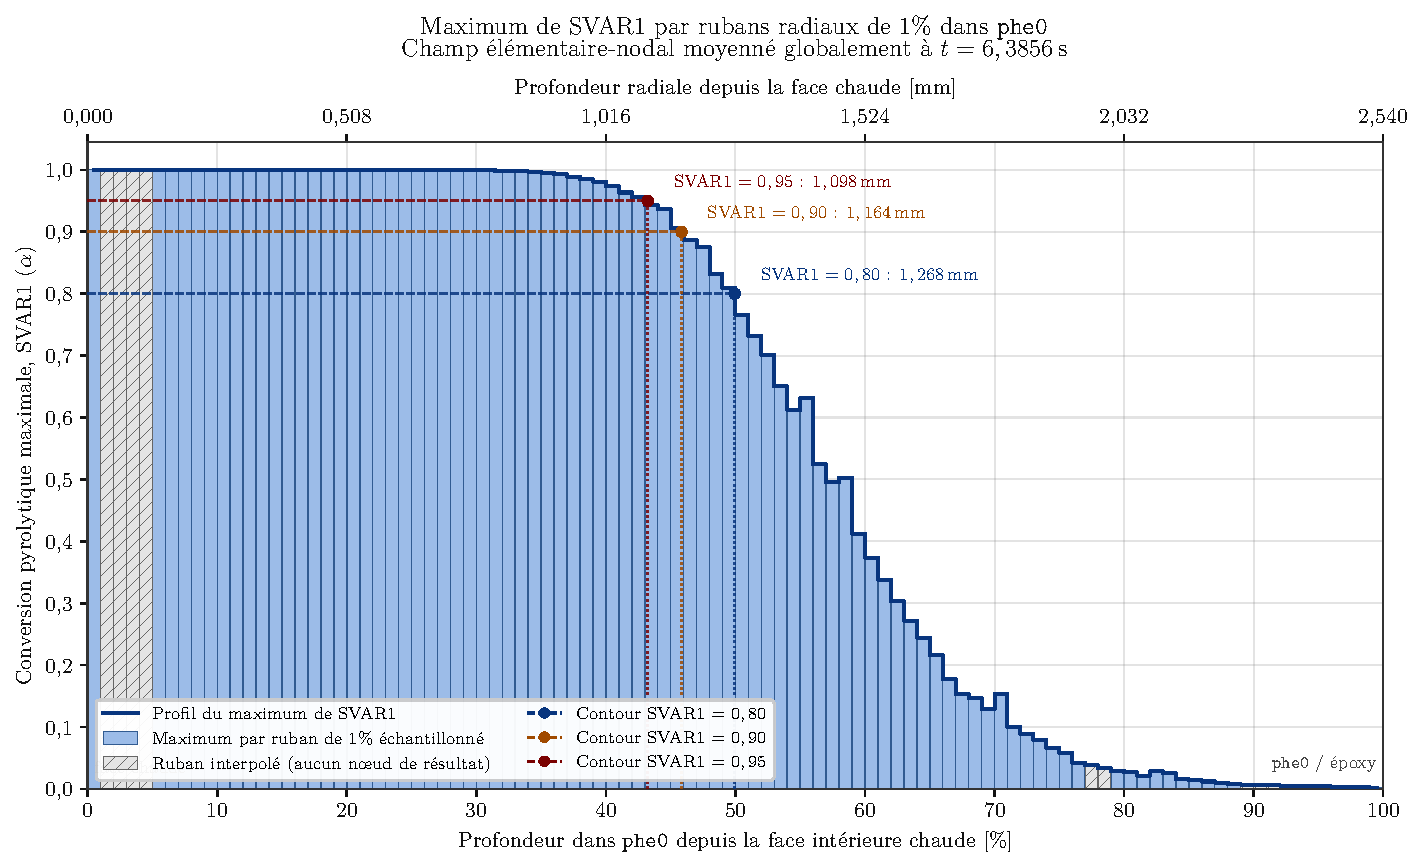
\includegraphics[width=0.98\textwidth]{../analysis/svar1_radial_profile_1pct_fr.pdf}
\caption{Maximum de \code{SVAR1} dans des rubans radiaux de 1\,\% de
\code{phe0}, au dernier état convergé. Les rubans hachurés ne contiennent aucun
nœud de résultat et sont interpolés linéairement.}
\label{fig:sim1-svar1-radial-fr}
\end{figure}

La figure~\ref{fig:sim1-svar1-radial-fr} représente l'enveloppe radiale maximale
du champ élémentaire-nodal moyenné globalement. Le maximum global atteint
\(\alpha=1\) : la zone proche de la face chaude est complètement convertie dans
le sens de la loi cinétique. Cela ne signifie toutefois ni que le char a été
enlevé, ni qu'un vide a été créé.

Les profondeurs des isoconversions sont données au
tableau~\ref{tab:sim1-front-results}. La zone à au moins 95\,\% de conversion
atteint \SI{1.098}{mm}, soit 43,2\,\% de l'épaisseur de \code{phe0}; le niveau
80\,\% atteint presque exactement la moitié de la couche.

\begin{table}[H]
\centering
\small
\renewcommand{\arraystretch}{1.15}
\begin{tabular}{M{0.15\textwidth}M{0.22\textwidth}M{0.22\textwidth}M{0.24\textwidth}}
\toprule
\textbf{Seuil \(\alpha_c\)} &
\textbf{Profondeur \(d_{\alpha_c}\) (mm)} &
\textbf{Fraction de \code{phe0}} &
\textbf{Vitesse apparente \(d_{\alpha_c}/t\) (\si{mm.s^{-1}})} \\
\midrule
0,80 & 1,26845 & 49,94\,\% & 0,19864 \\
0,90 & 1,16440 & 45,84\,\% & 0,18235 \\
0,95 & 1,09800 & 43,23\,\% & 0,17195 \\
\bottomrule
\end{tabular}~\\[1em]
\caption{Profondeur et vitesse moyenne apparente des fronts de conversion.}
\label{tab:sim1-front-results}
\end{table}

Les vitesses de la dernière colonne sont seulement les rapports
\(d_{\alpha_c}/t\). Elles supposent que le contour part de la face chaude à
\(t=0\) et donnent une vitesse moyenne de pénétration depuis l'allumage. Elles
ne sont pas des vitesses instantanées de front. Une vitesse de front rigoureuse
en \si{mm.s^{-1}} doit être calculée par différence entre les positions d'un
même contour sur plusieurs instants sauvegardés.

La largeur d'un ruban de la figure est \SI{25.4}{\micro m}, alors que
l'épaisseur radiale moyenne d'un élément de \code{phe0} est
\SI{0.318}{mm}. Les 100 barres améliorent la lecture et l'intégration du profil,
mais ne créent pas une résolution physique de 100 cellules. Seize rubans sans
nœud ont dû être interpolés; l'incertitude de localisation du front reste de
l'ordre d'une fraction d'élément et doit être mesurée par raffinement du
maillage.

\clearpage
\subsubsection{Évolution temporelle de la conversion}

\begin{figure}[H]
\centering
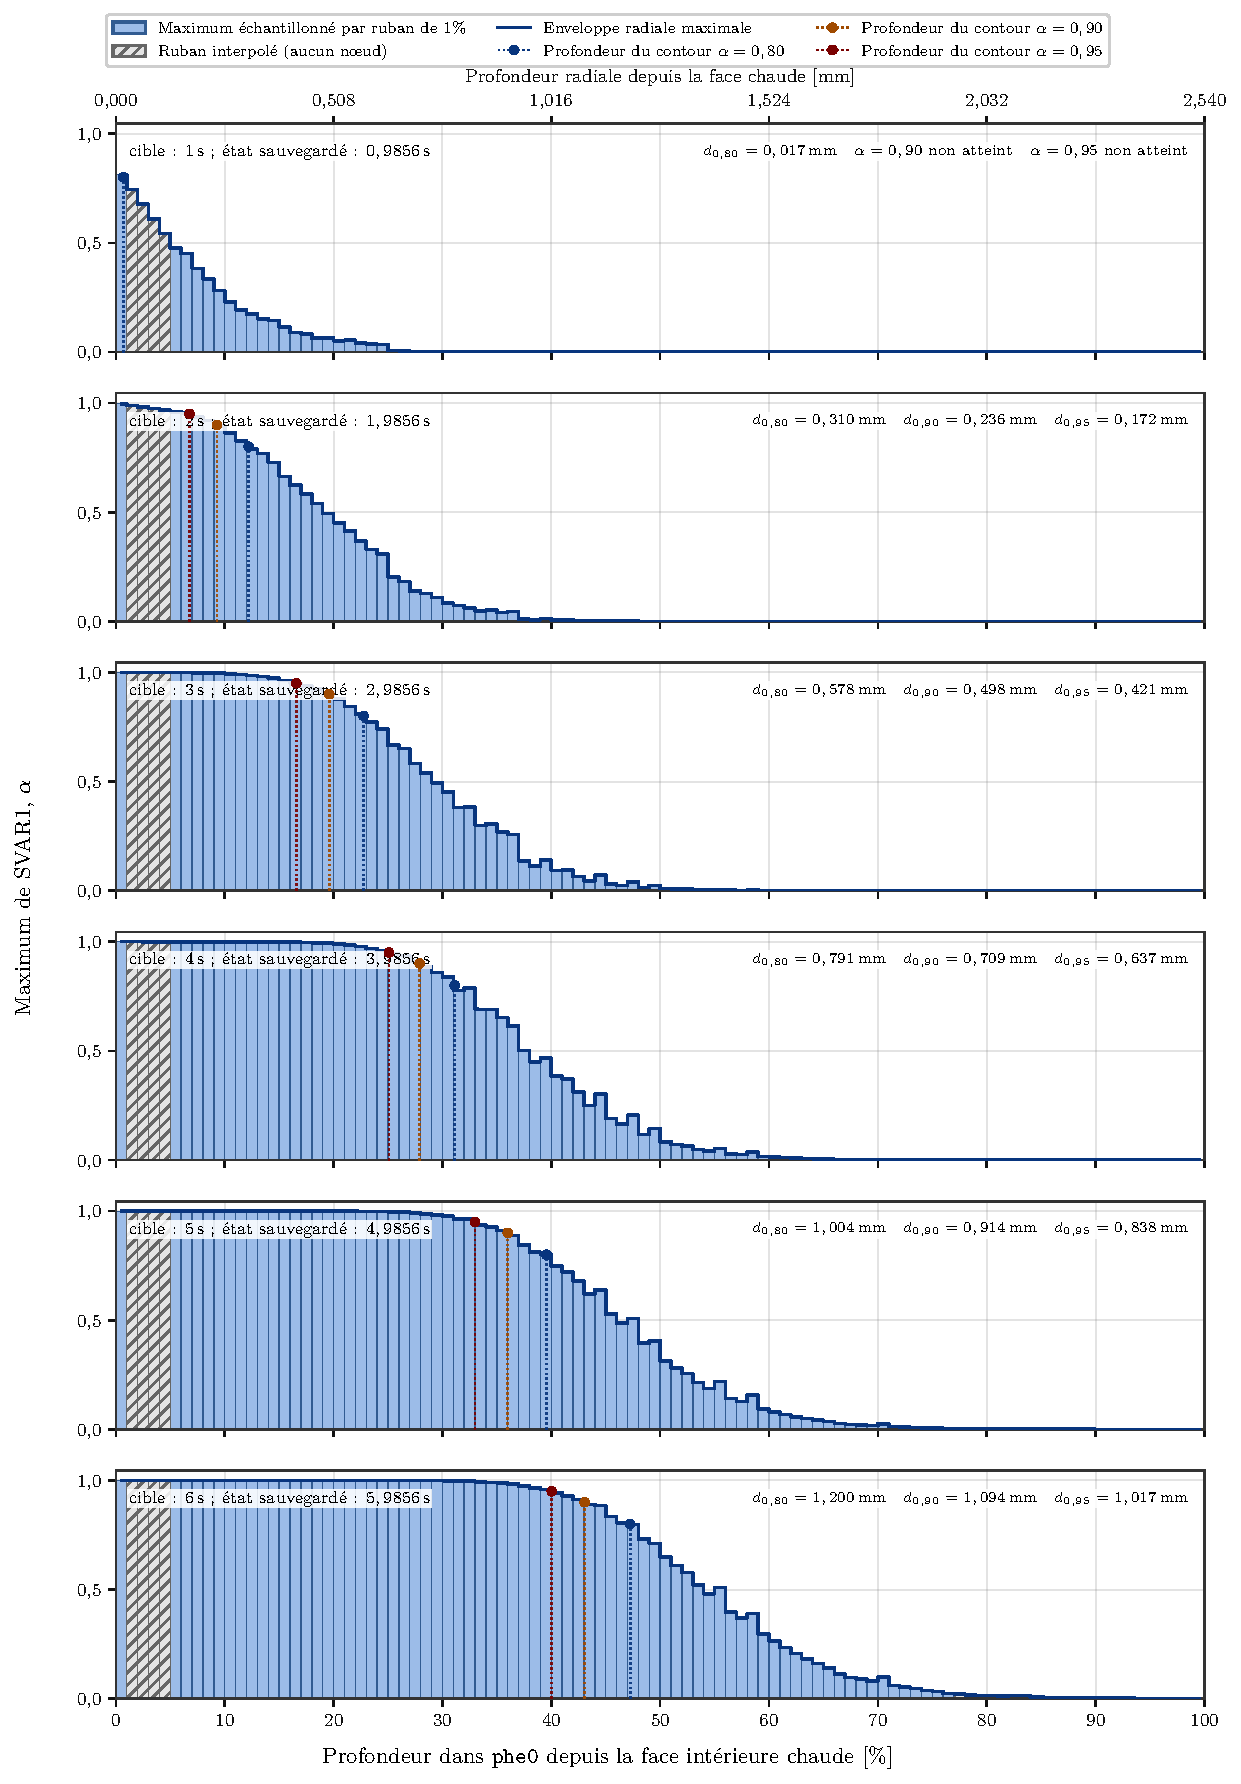
\includegraphics[height=0.80\textheight,width=0.96\textwidth,keepaspectratio]
{../analysis/svar1_time_profiles_1pct_fr.pdf}
\caption{Évolution du maximum radial de \code{SVAR1} dans \code{phe0}, pour les
états sauvegardés les plus proches de 1 à \SI{6}{s}. Les six graphes sont
empilés verticalement et utilisent les mêmes axes. Les traits pointillés et les
points repèrent les profondeurs des isoconversions 0,80, 0,90 et 0,95 lorsqu'elles
sont atteintes.}
\label{fig:sim1-svar1-time-fr}
\end{figure}
\clearpage

La figure~\ref{fig:sim1-svar1-time-fr} complète, sans remplacer, le profil du
dernier état convergé de la figure~\ref{fig:sim1-svar1-radial-fr}. Elle applique
exactement le même moyennage élémentaire-nodal et les mêmes rubans radiaux de
1\,\% aux six états sauvegardés les plus proches de \(t=1,\ldots,6~\si{s}\).
Les sorties disponibles précèdent chaque seconde entière de
\SI{0.014383}{s}; le temps réellement lu est indiqué dans chaque panneau afin
d'éviter de présenter une interpolation temporelle comme un résultat ANSYS.

Le tableau~\ref{tab:sim1-svar1-time} rassemble les valeurs utilisées pour les
annotations. À \SI{0.9856}{s}, la valeur maximale n'est encore que
\(\alpha=0{,}811\) et le contour 0,80 touche à peine la couche : les niveaux
0,90 et 0,95 ne sont pas encore atteints. Il s'agit d'une phase d'amorçage
thermique, et non d'un front déjà établi.

\begin{table}[H]
\centering
\small
\renewcommand{\arraystretch}{1.12}
\setlength{\tabcolsep}{4pt}
\begin{tabular}{M{0.12\textwidth}M{0.16\textwidth}M{0.14\textwidth}
                M{0.15\textwidth}M{0.15\textwidth}M{0.15\textwidth}}
\toprule
\textbf{Temps cible (s)} &
\textbf{Temps sauvegardé (s)} &
\textbf{\(\alpha_\mathrm{max}\)} &
\textbf{\(d_{0,80}\) (mm)} &
\textbf{\(d_{0,90}\) (mm)} &
\textbf{\(d_{0,95}\) (mm)} \\
\midrule
1 & 0,9856 & 0,81114 & 0,01691 & --- & --- \\
2 & 1,9856 & 0,99560 & 0,30979 & 0,23605 & 0,17200 \\
3 & 2,9856 & 0,99997 & 0,57818 & 0,49786 & 0,42106 \\
4 & 3,9856 & 1,00000 & 0,79069 & 0,70892 & 0,63735 \\
5 & 4,9856 & 1,00000 & 1,00433 & 0,91446 & 0,83788 \\
6 & 5,9856 & 1,00000 & 1,20013 & 1,09392 & 1,01716 \\
\bottomrule
\end{tabular}~\\[1em]
\caption{Progression temporelle des profondeurs d'isoconversion calculées sur
l'enveloppe radiale maximale.}
\label{tab:sim1-svar1-time}
\end{table}

Entre les états proches de 1 et \SI{2}{s}, le contour 0,80 avance à une vitesse
incrémentale moyenne de \SI{0.293}{mm.s^{-1}}. Cette vitesse diminue ensuite à
\SI{0.268}{mm.s^{-1}}, puis environ \SI{0.213}{mm.s^{-1}},
\SI{0.214}{mm.s^{-1}} et \SI{0.196}{mm.s^{-1}} sur les intervalles successifs.
Le contour 0,95, une fois apparu, ralentit de façon analogue, de
\SI{0.249}{mm.s^{-1}} entre 2 et \SI{3}{s} à
\SI{0.179}{mm.s^{-1}} entre 5 et \SI{6}{s}. La tendance générale est donc un
ralentissement du front, avec une petite variation non monotone compatible avec
les sous-pas, le lissage nodal et la résolution radiale du maillage.

Les profils montrent également qu'il n'existe pas une interface de pyrolyse
infiniment mince : une zone de transition large sépare le char presque
complètement converti du matériau encore vierge. À environ \SI{6}{s}, le contour
0,95 se trouve à \SI{1.017}{mm}, le contour 0,80 à \SI{1.200}{mm}, et la
conversion reste mesurable bien au-delà. Au dernier état disponible,
\SI{6.3856}{s}, ces profondeurs atteignent respectivement \SI{1.098}{mm} et
\SI{1.268}{mm}, ce qui prolonge sans discontinuité la tendance des six panneaux.

Pour le dimensionnement, une vitesse unique \(d/t\) masque donc à la fois le
délai d'amorçage et le ralentissement ultérieur. Toute extrapolation à la fin du
tir doit préciser le seuil de conversion choisi et employer, au minimum, une
vitesse incrémentale récente plutôt que de confondre conversion, profondeur de
char et récession géométrique. Enfin, comme chaque courbe est une enveloppe
radiale maximale, elle demeure conservative pour la conversion reconstruite
mais ne représente ni une moyenne volumique ni une profondeur d'ablation
réellement mesurée.

\subsubsection{Vitesse locale de pyrolyse \code{SVAR2}}

\code{SVAR2} est une vitesse de conversion locale en \si{s^{-1}}, différente
de la vitesse géométrique du tableau~\ref{tab:sim1-front-results}. Le maximum
global sur les partitions contenant \code{phe0} vaut
\[
  \boxed{\dot\alpha_\mathrm{max}=\SI{0.326660}{s^{-1}}.}
\]
Il apparaît à \SI{1.44221}{mm} de la face chaude, soit 56,78\,\% de
l'épaisseur, là où \(\alpha=0{,}54721\) et
\(T=\SI{956.67}{\degreeCelsius}=\SI{1229.82}{K}\). Cette position est
physiquement cohérente : près de la surface, le facteur \(1-\alpha\) est
presque nul parce que le matériau est déjà converti; plus profondément, la
température est trop faible pour activer rapidement la loi d'Arrhenius. Le
maximum de vitesse se place donc dans la zone de transition.

Sur le dernier sous-pas de \SI{0.05}{s}, ce maximum correspond à
\(\Delta\alpha\simeq0{,}01633\), bien inférieur à la limite numérique 0,05.
Le critère \code{UserMatTh} ne force donc pas une réduction supplémentaire du
dernier incrément. À ce point,
\[
  k_r=\frac{\dot\alpha}{1-\alpha}=\SI{0.7214}{s^{-1}},
  \qquad \tau_r=k_r^{-1}=\SI{1.386}{s}.
\]
Si la température restait artificiellement constante, il faudrait environ
\SI{3.05}{s} pour passer de \(\alpha=0{,}547\) à \(\alpha=0{,}95\).
La température locale continue en réalité d'évoluer : ce temps caractéristique
n'est donc pas une extrapolation jusqu'à la fin du tir.

Avec \(\rho_v-\rho_c\simeq\SI{550}{kg.m^{-3}}\) à cette température, la source
locale maximale suggérée pour la simulation 2 serait
\[
  \dot\omega'''_{g,\max}\simeq
  (\rho_v-\rho_c)\dot\alpha_\mathrm{max}
  =\SI{180}{kg.m^{-3}.s^{-1}}.
\]
Le puits thermique massique déjà appliqué par la simulation 1 vaut localement
\(-\Delta H_p\dot\alpha\simeq-\SI{136.5}{kW.kg^{-1}}\). La génération de gaz
est donc potentiellement importante, mais son transport, sa pression et son
échange de chaleur ne sont pas résolus dans le modèle courant.~\\
\subsubsection{Évolution temporelle de la vitesse locale}

\begin{figure}[H]
\centering
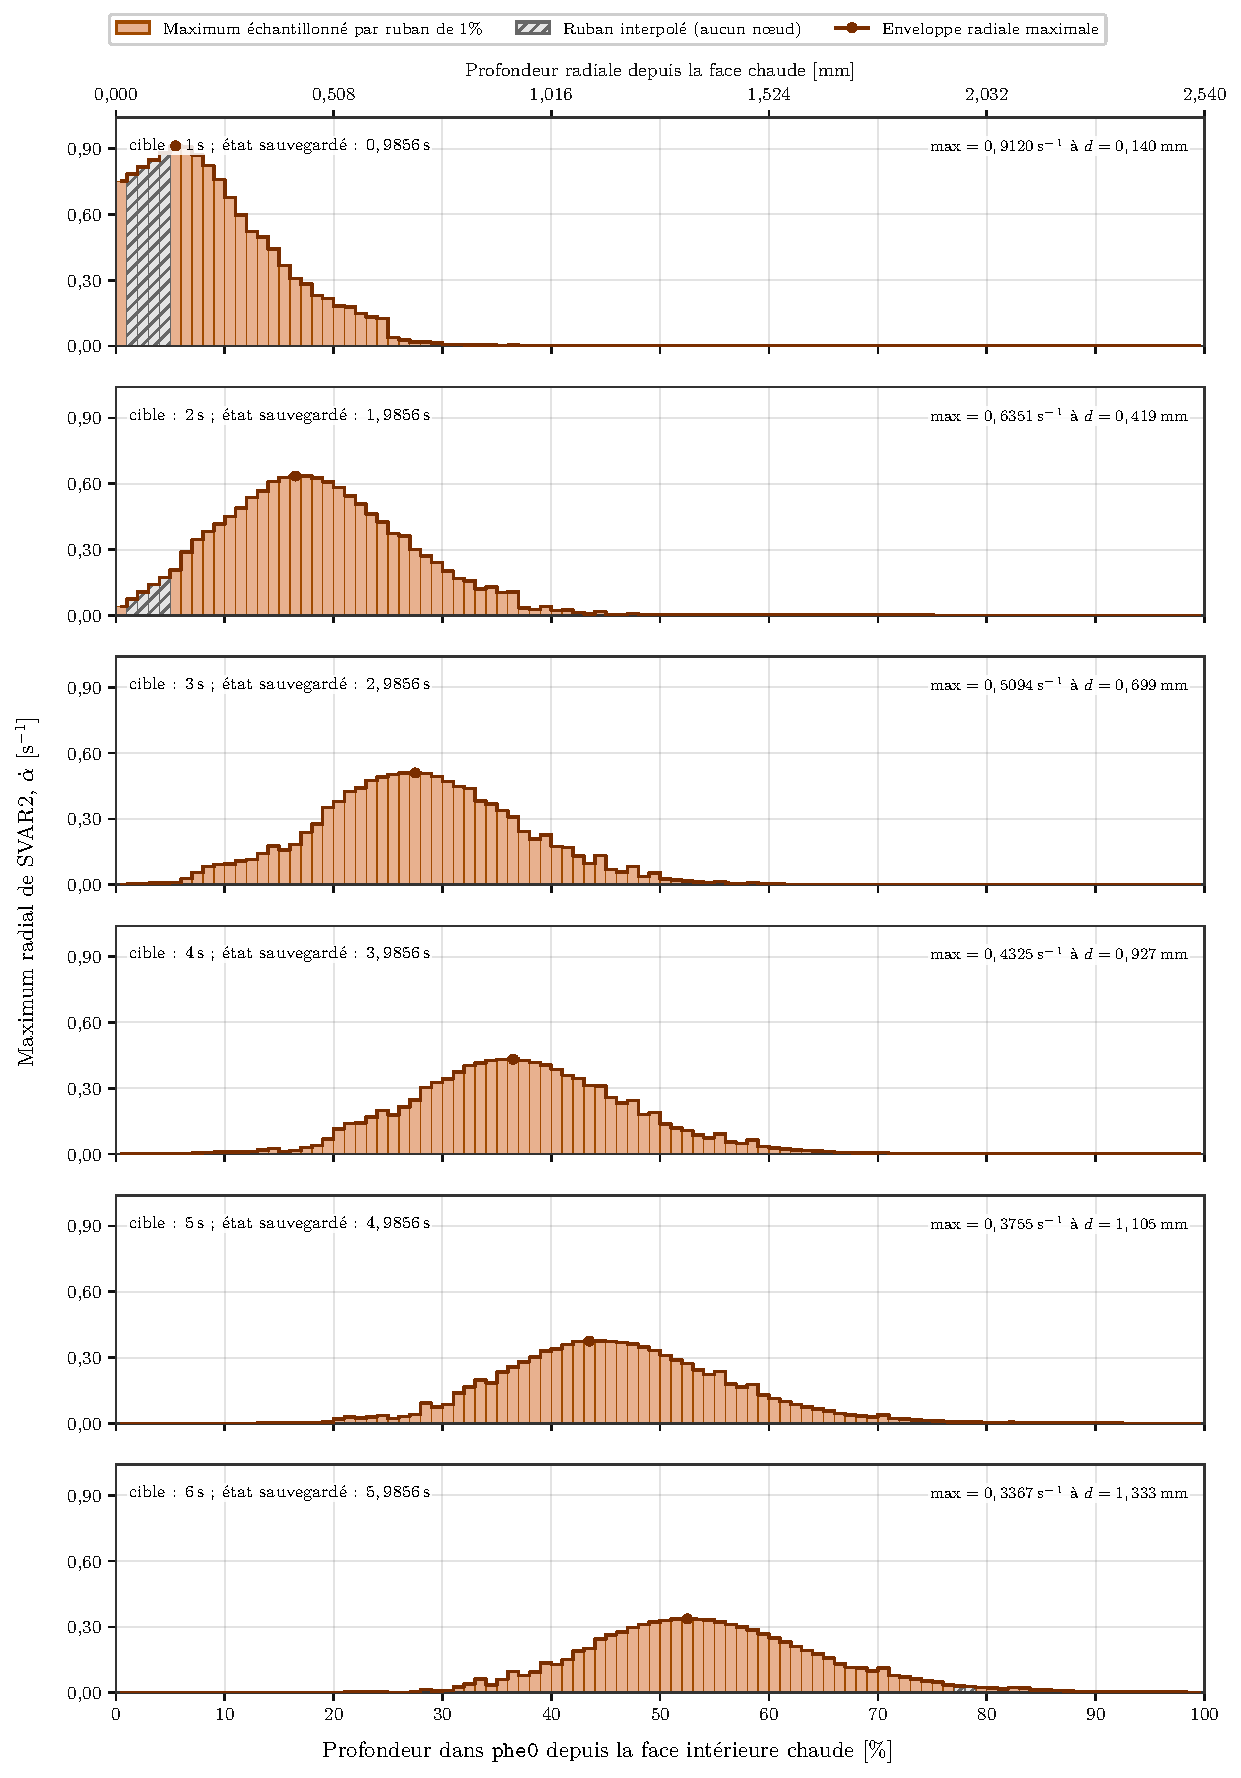
\includegraphics[height=0.80\textheight,width=0.96\textwidth,keepaspectratio]
{../analysis/svar2_radial_time_profiles_1pct_fr.pdf}
\caption{Évolution du maximum radial de \code{SVAR2} dans \code{phe0}, pour les
états sauvegardés les plus proches de 1 à \SI{6}{s}. Chaque panneau utilise la
même échelle verticale; les rubans hachurés ne contiennent aucun nœud de
résultat et sont interpolés linéairement.}
\label{fig:sim1-svar2-time-fr}
\end{figure}
\clearpage

La figure~\ref{fig:sim1-svar2-time-fr} applique à \code{SVAR2} la même étude
temporelle que la figure~\ref{fig:sim1-svar1-time-fr}. Le tableau
\ref{tab:sim1-svar2-time} montre simultanément la décroissance du maximum de
vitesse et son déplacement vers l'intérieur. Entre les états proches de 1 et
\SI{6}{s}, le maximum passe de \SI{0.9120}{s^{-1}} à
\SI{0.3367}{s^{-1}}, soit une diminution de 63,1\,\%, tandis que sa profondeur
passe de \SI{0.140}{mm} à \SI{1.333}{mm}.

\begin{table}[H]
\centering
\small
\renewcommand{\arraystretch}{1.12}
\begin{tabular}{M{0.18\textwidth}M{0.22\textwidth}M{0.25\textwidth}M{0.25\textwidth}}
\toprule
\textbf{Temps cible (s)} &
\textbf{Temps sauvegardé (s)} &
\textbf{\(\dot\alpha_\mathrm{max}\) (\si{s^{-1}})} &
\textbf{Profondeur du maximum (mm)} \\
\midrule
1 & 0,9856 & 0,9120 & 0,140 \\
2 & 1,9856 & 0,6351 & 0,419 \\
3 & 2,9856 & 0,5094 & 0,699 \\
4 & 3,9856 & 0,4325 & 0,927 \\
5 & 4,9856 & 0,3755 & 1,105 \\
6 & 5,9856 & 0,3367 & 1,333 \\
\bottomrule
\end{tabular}~\\[1em]
\caption{Migration temporelle du maximum radial de vitesse de pyrolyse.}
\label{tab:sim1-svar2-time}
\end{table}

La trajectoire n'est pas une récession géométrique. Elle repère le lieu où le
produit du facteur d'Arrhenius et de la fraction vierge restante est maximal.
La face chaude se sature rapidement, donc \(1-\alpha\) y devient presque nul;
le maximum de \(\dot\alpha\) se déplace alors vers du matériau plus profond,
encore partiellement vierge mais suffisamment chaud. Le ralentissement du
maximum traduit l'atténuation thermique avec la profondeur et non l'arrêt de
la pyrolyse. Il explique aussi pourquoi la source de gaz de la simulation 2
devra être volumique et mobile : l'emploi du seul taux à la surface
sous-estimerait fortement la production dans la zone de transition après les
premières secondes.

\subsubsection{Dépendance axiale sur la face intérieure chaude}

La coordonnée axiale est mesurée depuis le plan inférieur du tronçon maillé,
\(y=\SI{0.9144}{m}\), sur sa longueur de \SI{50}{mm}. Dans chaque ruban axial
de 1\,\%, les figures suivantes retiennent le maximum des nœuds de la face
intérieure chaude de \code{phe0}. Cette restriction évite de remplacer un
ruban sans nœud de surface par un nœud froid situé plus profondément. Les
valeurs sont obtenues par le moyennage élémentaire-nodal natif de DPF, puis par
fusion des nœuds globaux dupliqués aux frontières DMP. Quatre-vingt-trois
rubans sur 100 sont directement échantillonnés; les 17 autres sont clairement
hachurés et interpolés entre leurs voisins.

\clearpage
\begin{figure}[H]
\centering
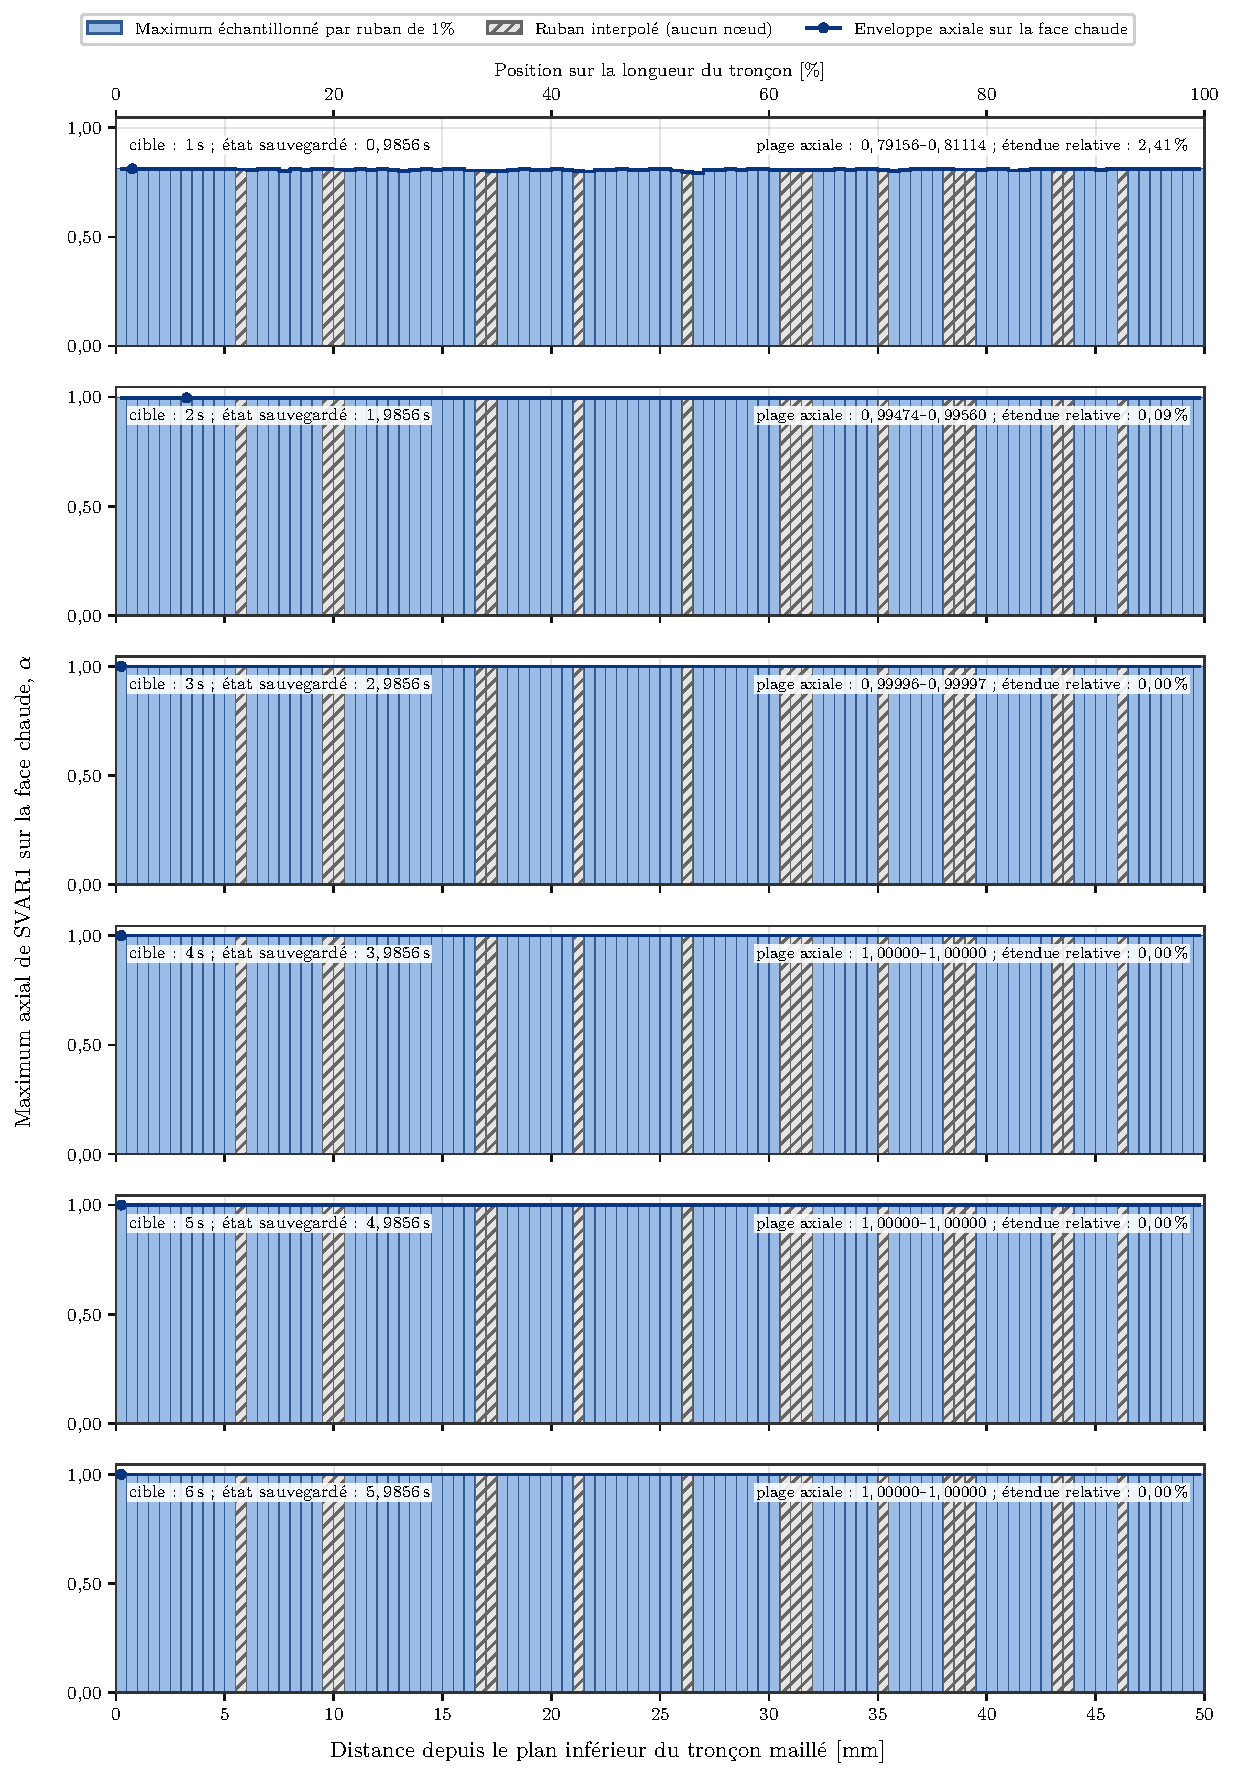
\includegraphics[height=0.80\textheight,width=0.96\textwidth,keepaspectratio]
{../analysis/svar1_axial_time_profiles_1pct_fr.pdf}
\caption{Dépendance axiale de \code{SVAR1} sur la face intérieure chaude de
\code{phe0}, depuis le plan inférieur du tronçon maillé. Les six panneaux
emploient la même échelle \(0\leq\alpha\leq1\).}
\label{fig:sim1-svar1-axial-fr}
\end{figure}
\clearpage

\begin{figure}[H]
\centering
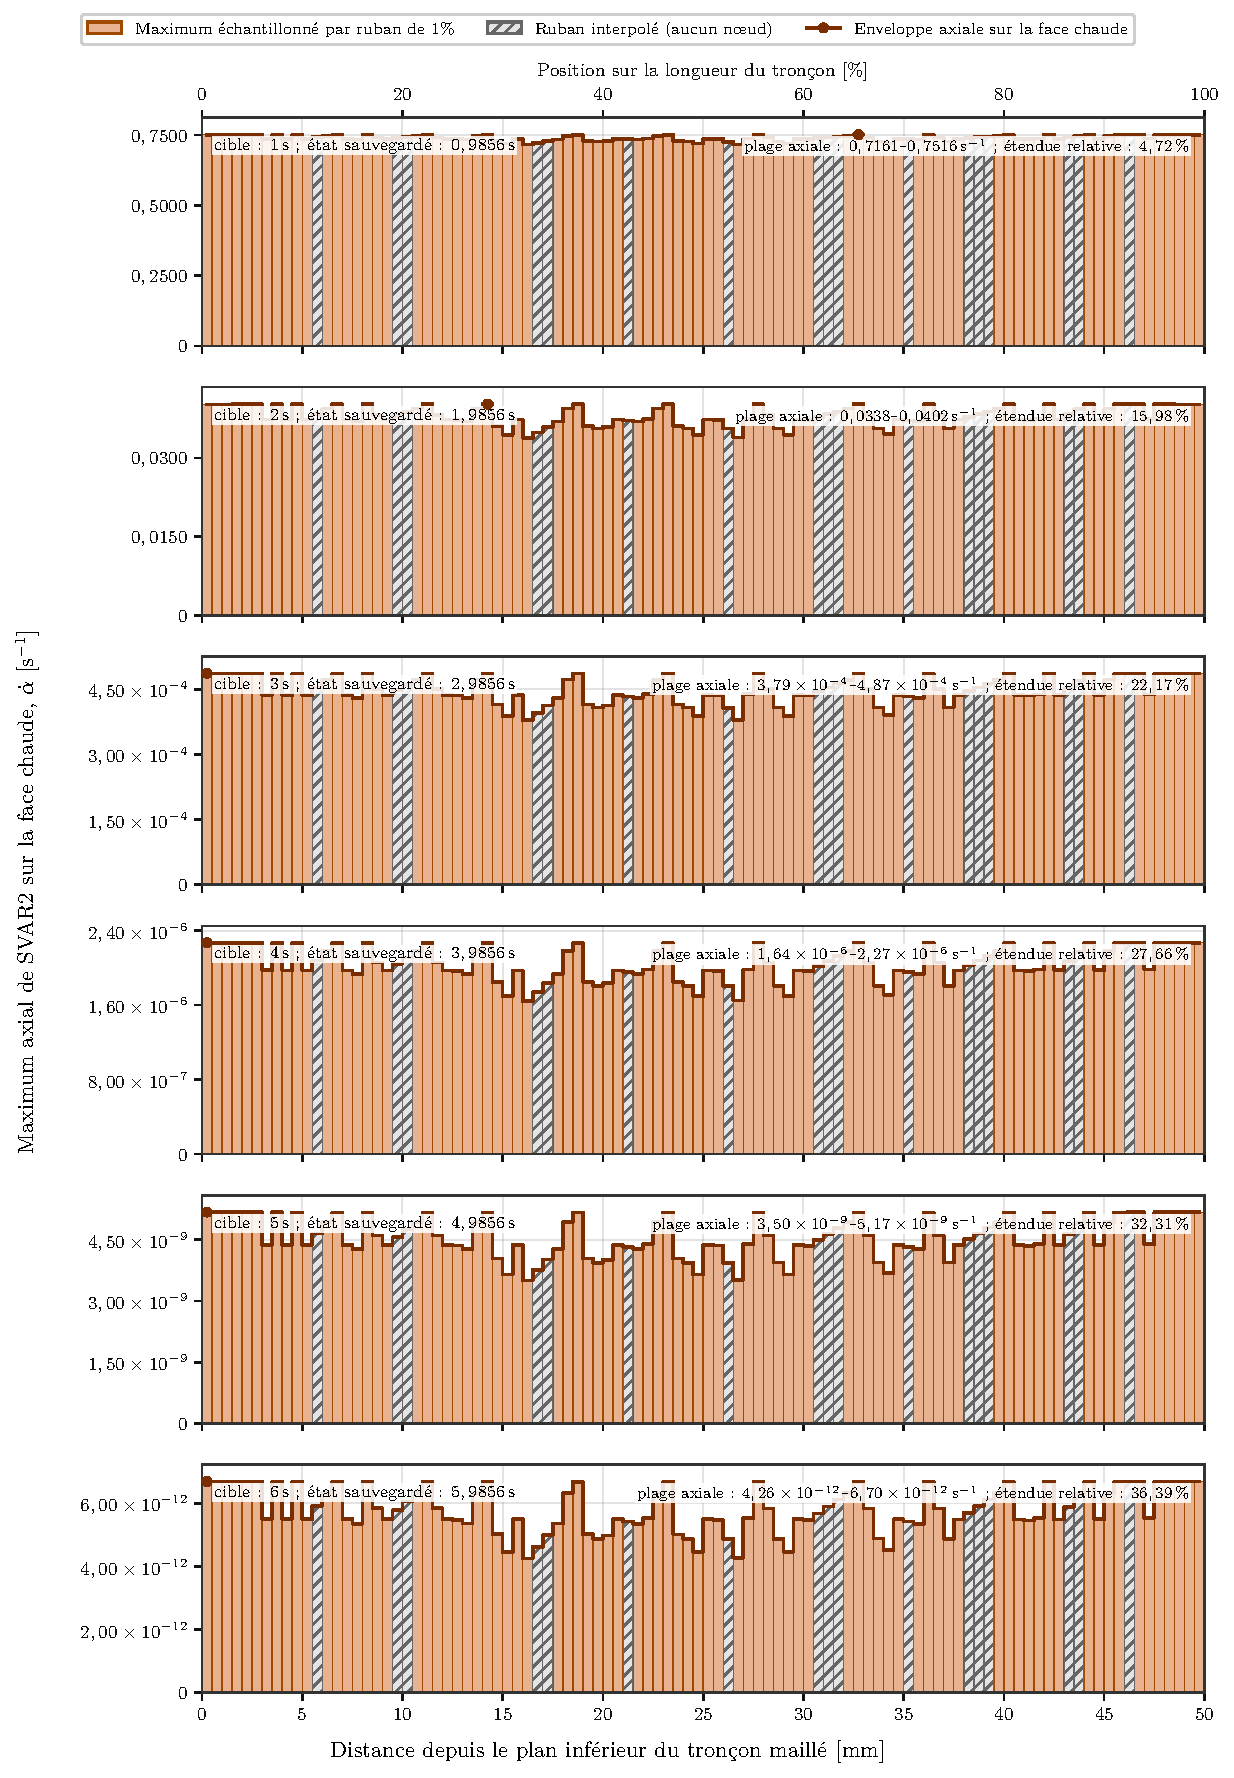
\includegraphics[height=0.80\textheight,width=0.96\textwidth,keepaspectratio]
{../analysis/svar2_axial_time_profiles_1pct_fr.pdf}
\caption{Dépendance axiale de \code{SVAR2} sur la face intérieure chaude de
\code{phe0}. L'échelle verticale est indépendante dans chaque panneau afin de
rendre visibles les faibles taux tardifs; les valeurs absolues, et non les
hauteurs relatives des barres entre panneaux, doivent être comparées.}
\label{fig:sim1-svar2-axial-fr}
\end{figure}
\clearpage

La figure~\ref{fig:sim1-svar1-axial-fr} montre une conversion de surface
presque uniforme. À \SI{0.9856}{s}, \(\alpha\) varie de 0,79156 à 0,81114,
soit une étendue relative de 2,41\,\%. À \SI{1.9856}{s}, la plage se resserre
à 0,99474--0,99560; à \SI{2.9856}{s}, elle vaut
0,999959--0,999968. La face chaude est numériquement entièrement convertie à
partir de l'état proche de \SI{4}{s}. Cela signifie « char complètement
formé » selon la variable d'état, pas « matière enlevée ».

La figure~\ref{fig:sim1-svar2-axial-fr} apporte l'information complémentaire.
Le taux sur la face chaude vaut encore
\(\SIrange{0.7161}{0.7516}{s^{-1}}\) près de \SI{1}{s}, mais tombe à
\(\SIrange{0.03382}{0.04025}{s^{-1}}\) près de \SI{2}{s}, puis à
\(\SIrange{3.79e-4}{4.87e-4}{s^{-1}}\) près de \SI{3}{s}. Il devient inférieur
à \SI{2.3e-6}{s^{-1}} près de \SI{4}{s} et pratiquement nul ensuite. Cette
chute abrupte est la conséquence attendue du facteur \(1-\alpha\) : la surface
n'a presque plus de matière vierge à convertir, alors que la figure
\ref{fig:sim1-svar2-time-fr} confirme que le front volumique reste actif plus
profondément.

L'étendue axiale relative de \code{SVAR2} augmente de 4,72\,\% à \SI{1}{s} à
36,39\,\% à \SI{6}{s}, mais cette croissance est trompeuse si elle est lue
seule : le dénominateur a diminué d'environ onze ordres de grandeur. Les
variations tardives sont donc négligeables en valeur absolue et reflètent
surtout le maillage, le lissage nodal et la saturation numérique. Sous les
conditions aux limites uniformes de ce tronçon central, les deux figures
valident l'hypothèse d'une réponse axialement quasi uniforme. Elles soutiennent
l'emploi futur d'un modèle axisymétrique beaucoup moins coûteux pour la zone
centrale, mais ne disent rien des extrémités, de la tuyère, des joints ou des
variations réelles du flux de combustion.

\subsubsection{Encadrement de la conversion et du dégazage potentiel}

Deux reconstructions simples permettent d'encadrer l'ordre de grandeur, sans
prétendre fournir une incertitude statistique. La reconstruction basse pose
\(\alpha=0{,}95\) entre la face chaude et le contour à \SI{1.098}{mm}, puis
\(\alpha=0\) au-delà. En tenant compte de la géométrie cylindrique, elle donne
\(\bar\alpha_\mathrm{bas}=0{,}408\). L'intégration de l'enveloppe maximale des
100 rubans donne
\(\bar\alpha_\mathrm{haut}=0{,}581\). Le tableau~\ref{tab:sim1-mass-bracket}
emploie ensuite le rendement gazeux nominal \(Y_g=0{,}47\).

\begin{table}[H]
\centering
\small
\renewcommand{\arraystretch}{1.15}
\begin{tabular}{L{0.31\textwidth}M{0.20\textwidth}M{0.20\textwidth}M{0.18\textwidth}}
\toprule
\textbf{Reconstruction} &
\(\boldsymbol{\bar\alpha}\) &
\textbf{Épaisseur convertie équivalente} &
\textbf{Gaz potentiel} \\
\midrule
Basse : front 95\,\% en échelon & 0,408 & \SI{1.04}{mm} &
\SI{0.943}{kg} moteur complet; \SI{25.8}{g} tronçon \\
Haute : enveloppe radiale maximale & 0,581 & \SI{1.48}{mm} &
\SI{1.340}{kg} moteur complet; \SI{36.6}{g} tronçon \\
\bottomrule
\end{tabular}~\\[1em]
\caption{Encadrement d'ingénierie de la conversion et de la masse gazeuse
potentielle à \(t=\SI{6.3856}{s}\).}
\label{tab:sim1-mass-bracket}
\end{table}

Ces valeurs supposent que le profil est représentatif sur toute la
circonférence et toute la longueur, puis utilisent la masse complète de
\code{phe0}, \SI{4.911}{kg}. Pour le modèle maillé, la longueur est seulement
\SI{50}{mm} et la masse initiale correspondante vaut environ \SI{0.134}{kg}.
La reconstruction haute emploie des maxima radiaux : elle est volontairement
conservative pour une moyenne. La reconstruction basse n'est pas une borne
mathématique de la solution 3D, car la figure ne contient pas les minima
circonférentiels et axiaux. Enfin, la « masse gazeuse potentielle » est la masse
qui serait libérée selon la loi de densité; le solveur ne démontre pas que cette
masse a effectivement quitté le solide.

\subsubsection{Conséquences physiques et conséquences pour la conception}

\begin{enumerate}[leftmargin=2.2em,label=\textbf{\arabic*.}]
  \item \textbf{Marge du liner interne.} Une épaisseur d'environ
  \SIrange{1.10}{1.27}{mm} est déjà convertie à 80--95\,\%, et le maximum de
  \code{SVAR2} se situe à \SI{1.44}{mm}. Le front est encore actif et progresse
  vers l'époxy. La différence \(2{,}54-d_{\alpha_c}\) ne peut pas être traitée
  directement comme une marge d'ablation, mais elle montre que la première
  couche est fortement sollicitée avant la fin prévue du tir.

  \item \textbf{Époxy critique.} Le modèle prédit
  \SI{453}{\degreeCelsius} dans une couche d'époxy pourtant supposée inerte et
  liée. Cette valeur dépasse le domaine de sa table thermique. Le modèle ne
  permet donc pas d'affirmer que l'adhésion \code{phe0--epo} ou
  \code{epo--phe1} subsiste. Une caractérisation de l'époxy, une barrière
  thermique plus épaisse ou un adhésif haute température doivent être étudiés
  avant de considérer la liaison comme sûre.

  \item \textbf{Aluminium protégé à court terme seulement.} Le tronçon central
  idéal conserve l'aluminium à environ \SI{22}{\degreeCelsius} à
  \SI{6.39}{s}. C'est favorable, mais cela ne couvre ni l'échauffement retardé
  après extinction, ni les ponts thermiques, ni les extrémités et interfaces de
  tuyère. Une phase de refroidissement transitoire doit être ajoutée pour
  rechercher le maximum retardé de la température de l'aluminium.

  \item \textbf{Dégazage non négligeable.} La valeur de \code{SVAR2} implique
  une source locale de gaz élevée. Sans transport poreux, la simulation ne peut
  prédire ni la pression interne du char, ni le refroidissement par soufflage,
  ni un risque de délamination assistée par les gaz. Ces phénomènes motivent
  directement la simulation 2.

  \item \textbf{Résolution du front.} Huit éléments sur \SI{2.54}{mm} donnent
  seulement trois à quatre couches d'éléments dans la zone de transition
  principale. Un calcul avec 16 puis 24 couches radiales doit comparer
  \(d_{0.8}\), \(d_{0.95}\), \(\dot\alpha_\mathrm{max}\) et la température de
  l'époxy.

  \item \textbf{Limite du tronçon central.} Le maillage de \SI{50}{mm}
  représente correctement une zone uniforme de mi-longueur, mais pas les
  concentrations de flux ou les chemins conductifs des extrémités. Les masses
  du tableau~\ref{tab:sim1-mass-bracket} ne peuvent être étendues au moteur
  complet que si l'uniformité axiale est vérifiée.
\end{enumerate}

\subsubsection{Comparaison à la réalité et sens des bornes}

Il n'existe actuellement ni courbe TGA/DSC/LFA du phénolique réellement
fabriqué, ni thermocouple d'essai moteur, ni mesure post-tir de masse, de
profondeur de char ou de récession. Il serait donc incorrect d'annoncer un
accord quantitatif avec la réalité. La comparaison possible à ce stade porte
sur les mécanismes : les modèles d'ablateurs carbonisants vérifiés par la NASA
incluent la conduction, la décomposition, la circulation des gaz de pyrolyse,
les échanges gaz-solide, l'érosion thermochimique et le déplacement de la
surface~\cite{ewing2013,amar2010,amar2016}. La simulation 1 ne représente que
la conduction, la cinétique locale, les propriétés vierge/char et le puits
endothermique.

\begin{table}[H]
\centering
\footnotesize
\renewcommand{\arraystretch}{1.18}
\begin{tabular}{L{0.25\textwidth}L{0.34\textwidth}L{0.31\textwidth}}
\toprule
\textbf{Hypothèse ou omission} & \textbf{Effet physique absent} &
\textbf{Biais probable} \\
\midrule
\(T_g\) et \(h_\mathrm{in}\) constants dès \(t=0\) &
Montée d'allumage et décroissance de pression absentes &
Tendance haute si le tir réel présente des rampes; direction inconnue si le
flux réel ou le rayonnement particulaire est supérieur. \\
Pas de gaz de pyrolyse mobile &
Pas de soufflage pariétal, d'enthalpie advectée ni de pression poreuse &
Souvent une tendance haute pour le flux net pénétrant, mais pas une borne
unilatérale pour la température interne. \\
Pas d'oxydation, d'érosion ni de particules &
Pas de consommation thermochimique ou mécanique du char &
Borne basse pour la récession et la perte géométrique. \\
Char conservé et aucun élément supprimé &
La surface ne recule jamais &
Récession calculée exactement nulle : borne basse imposée par le modèle. \\
Contacts parfaitement liés &
Ni interstice, ni délamination, ni résistance évolutive &
Tendance haute pour la transmission thermique idéale, mais vision trop
optimiste de l'intégrité de l'adhésif. \\
Propriétés et cinétique non calibrées &
Grade, fibres, rendement en char et réactions multiples inconnus &
Pas de sens de biais défendable; cette incertitude peut dominer toutes les
autres. \\
Profil radial maximal &
Enveloppe, pas moyenne volumique &
Borne haute d'ingénierie pour la conversion moyenne reconstruite. \\
\bottomrule
\end{tabular}~\\[1em]
\caption{Sens attendu des principaux biais par rapport à un tir réel.}
\label{tab:sim1-reality-bounds}
\end{table}

Pour la \emph{récession géométrique}, la borne basse du modèle courant est donc
\SI{0}{mm}. Une borne haute simple consiste à supposer que toute l'épaisseur
convertie équivalente, environ \SIrange{1.0}{1.5}{mm}, est également arrachée;
elle est volontairement sévère car 52--56\,\% de la masse condensée subsiste
sous forme de char selon les tables actuelles. La réalité peut se situer entre
ces valeurs si le char reste partiellement attaché, mais une forte oxydation ou
une érosion mécanique peut invalider cet encadrement. Seul un tir instrumenté
et une mesure post-tir peuvent le fermer.

Les priorités de validation sont donc : (i) caractériser le phénolique et
l'époxy réels par TGA, DSC et LFA, méthodes explicitement utilisées par la NASA
pour la masse résiduelle, la capacité calorifique et la diffusivité
thermique~\cite{nasa-testing}; (ii) mesurer \(T_g(t)\), la pression et des
températures aux interfaces et sur l'aluminium pendant un tir; (iii) mesurer la
masse, l'épaisseur résiduelle et la profondeur de char après tir; (iv) prolonger
le calcul jusqu'à \SI{7}{s} puis pendant le refroidissement; et (v) réaliser des
études de sensibilité sur \(h_\mathrm{in}\), \(A\), \(E_a\), \(\Delta H_p\),
les propriétés du char, les contacts, le pas de temps et le maillage.

% ============================================================================
\clearpage
\section{Simulation 2 : Dégazage et Suppression d'Éléments dans Mechanical}

\subsection{Théorie Proposée et Dérivation}

\subsubsection{Bilan de Masse du Solide et Génération de Gaz}

La simulation 2 conserve la cinétique de la simulation 1, mais distingue le
résidu solide des produits gazeux. Sur un volume initial, la diminution de masse
condensée est la source de gaz :
\begin{equation}
  \frac{\pd\rho_s}{\pd t}=-\dot\omega'''_g,
  \qquad
  \dot\omega'''_g=(\rho_v-\rho_c)\dot\alpha.
  \label{eq:solid-mass-sim2}
\end{equation}
Le rendement gazeux final du modèle à une réaction vaut donc
\begin{equation}
  Y_g=\frac{\rho_v-\rho_c}{\rho_v}=1-\frac{\rho_c}{\rho_v}.
  \label{eq:gas-yield}
\end{equation}
Avec les tables actuelles, \(Y_g\) varie de 0,44 à 0,48; une valeur nominale
\(Y_g=0{,}47\) est cohérente avec le modèle, mais doit être confirmée par la
masse résiduelle TGA.

Dans un modèle complet d'ablateur poreux, la conservation de masse du gaz est
\begin{equation}
  \frac{\pd(\phi\rho_g)}{\pd t}
  +\vect\nabla\cdot(\rho_g\vect u_g)=\dot\omega'''_g,
  \label{eq:gas-mass-full}
\end{equation}
où \(\phi\) est la porosité et \(\vect u_g\) la vitesse superficielle. Pour un
écoulement lent dans le char, la loi de Darcy et le gaz parfait donnent
\begin{equation}
  \vect u_g=-\frac{K(\alpha,T)}{\mu_g}\vect\nabla p_g,
  \qquad
  \rho_g=\frac{p_g M_g}{R T_g}.
  \label{eq:darcy-ideal}
\end{equation}
Les codes de réponse de matériaux ablatifs tels que CHAR résolvent des versions
couplées de ces bilans de masse et d'énergie~\cite{amar2010,amar2016,ewing2013}.
Un élément thermique standard de Mechanical n'a toutefois aucun degré de liberté
de pression. \code{UserMatTh} ne peut donc pas, à elle seule, résoudre
l'équation~\eqref{eq:gas-mass-full}. Rester dans Mechanical impose soit un
élément utilisateur multiphysique beaucoup plus lourd, soit un modèle réduit.

\subsubsection{Fermeture radiale réduite compatible avec Mechanical}

Le modèle proposé considère que les gaz formés dans \code{phe0} s'évacuent
rapidement vers la paroi chaude et que leur stockage est négligeable. En
axisymétrie cylindrique, le flux massique de gaz atteignant la surface de rayon
\(r_s\) est alors obtenu directement par intégration de la source :
\begin{equation}
  \boxed{\dot m''_g(r_s)=\frac{1}{r_s}
  \int_{r_s}^{R_0}\dot\omega'''_g(r)\,r\,\dd r,}
  \label{eq:radial-gas-flux}
\end{equation}
où \(R_0\) est la limite externe de \code{phe0}. Cette expression provient du
bilan \(2\pi r_sL\dot m''_g=\int_{r_s}^{R_0}2\pi rL
\dot\omega'''_g\dd r\). Elle conserve la masse gazeuse globale même sans
pression résolue.

Le gaz emporte une enthalpie sensible. Une fermeture locale minimale ajoute à
l'équation du solide
\begin{equation}
  \dot q_{m,g}=-\frac{\dot\omega'''_g}{\rho_s}
  c_{p,g}(T-T_\mathrm{ref}).
  \label{eq:gas-local-sink}
\end{equation}
Ce terme ne doit être utilisé que si \(\Delta H_p\) ne contient pas déjà cette
enthalpie; sinon il y aurait double comptage. Une formulation plus fidèle ajoute
\(-\vect\nabla\cdot(\dot m''_g h_g)\) au bilan d'énergie, comme dans les modèles
de réponse matériau~\cite{ewing2013,amar2010}.

\subsubsection{Réduction du flux convectif par soufflage}

Le dégazage vers la chambre crée un soufflage opposé au transfert de chaleur.
Dans un film gazeux plan, stationnaire, à propriétés constantes, l'équation
d'énergie sans source s'écrit
\begin{equation}
  \dot m''_g c_{p,g}\frac{\dd T}{\dd y}
  =k_g\frac{\dd^2T}{\dd y^2}.
\end{equation}
En intégrant entre la paroi et le bord du film puis en exprimant l'épaisseur par
le coefficient sans soufflage \(h_0=k_g/\delta\), on obtient la correction
classique sous la forme
\begin{equation}
  B_h=\frac{\dot m''_g c_{p,g}}{h_0},\qquad
  F(B_h)=\frac{B_h}{\exp(B_h)-1},
\end{equation}
\begin{equation}
  \boxed{q''_\mathrm{conv}=h_0F(B_h)(T_g-T_s).}
  \label{eq:blowing}
\end{equation}
Comme \(F(0)=1\) et \(F(B_h)<1\) pour \(B_h>0\), le modèle revient à la
convection actuelle sans dégazage et réduit progressivement le flux lorsque la
production de gaz augmente. Cette loi est une fermeture d'ingénierie; elle ne
remplace pas un calcul de couche limite et doit être calibrée sur pression,
composition du propergol et essai.

\subsubsection{Bilan de surface, récession et critère de suppression}

La pyrolyse produit du char; elle ne retire pas automatiquement ce char. La
récession demande un second mécanisme --- oxydation, sublimation ou érosion
mécanique --- et un bilan à la surface :
\begin{equation}
  q''_\mathrm{conv}+q''_\mathrm{rad}
  =q''_\mathrm{cond}+\dot m''_g\Delta h_g
   +\dot m''_\mathrm{abl}H_\mathrm{eff}.
  \label{eq:surface-balance}
\end{equation}
En l'absence de données chimiques suffisantes, une loi énergétique bornée est
proposée :
\begin{equation}
  \dot m''_\mathrm{abl}=
  \max\left[0,
  \frac{q''_\mathrm{conv}+q''_\mathrm{rad}-q''_\mathrm{cond}
  -\dot m''_g\Delta h_g}{H_\mathrm{eff}}\right],
  \qquad
  \dot s=\frac{\dot m''_\mathrm{abl}}{\rho_c}.
  \label{eq:recession}
\end{equation}
La profondeur récessée est \(s(t)=\int_0^t\dot s\dd t\). Les éléments de
\code{phe0} sont organisés en bandes radiales; une bande n'est supprimée que
lorsque \(s\) franchit son épaisseur cumulée. Le critère est donc la récession
intégrée, éventuellement assortie de \(\alpha\ge0{,}99\), mais jamais
\(\alpha=1\) seul.

Dans MAPDL, \code{EKILL} multiplie la contribution d'un élément par un facteur
quasi nul; l'élément reste dans le maillage. Un élément thermique mort n'apporte
plus de capacité ni de charge, et ses variables d'état sont remises à zéro lors
de la mort~\cite{ansys-birthdeath,ansys-ekill}. Toute énergie et masse résiduelles
doivent donc être enregistrées avant \code{EKILL} et incluses dans un bilan.
Après chaque mort de bande, la convection chaude et les éléments surfaciques
doivent être transférés à la nouvelle face exposée. Avec seulement huit couches
dans \code{phe0}, la récession progresserait par sauts d'environ
\SI{0.318}{mm}; une étude de retrait crédible devrait viser 20 à 40 bandes
radiales, ou démontrer que cette marche est suffisamment petite.

\begin{figure}[H]
\centering
\begin{tikzpicture}[font=\sffamily\small,>=Latex,node distance=8mm and 9mm,
  block/.style={draw=B,very thick,rounded corners=7pt,fill=b!10,
    align=center,text width=34mm,minimum height=13mm},
  special/.style={draw=phenolicA,very thick,rounded corners=7pt,fill=phenolicB!20,
    align=center,text width=34mm,minimum height=13mm},
  kill/.style={draw=r,very thick,rounded corners=7pt,fill=red!8,
    align=center,text width=34mm,minimum height=13mm},
  arr/.style={-Latex,very thick,draw=black!60}]
  \node[block] (pyro) {pyrolyse locale\\\(\alpha,\dot\omega'''_g\)};
  \node[block,right=of pyro] (gas) {flux gazeux radial\\\(\dot m''_g\)};
  \node[special,right=of gas] (blow) {soufflage et enthalpie\\\(F(B_h),\Delta h_g\)};
  \node[block,below=of blow] (surface) {bilan de surface\\\(\dot m''_\mathrm{abl}\)};
  \node[special,left=of surface] (recession) {récession intégrée\\\(s(t)\)};
  \node[kill,left=of recession] (ekill) {franchissement de bande\\\code{EKILL}};
  \draw[arr] (pyro)--(gas); \draw[arr] (gas)--(blow);
  \draw[arr] (blow)--(surface); \draw[arr] (surface)--(recession);
  \draw[arr] (recession)--(ekill);
  \draw[arr] (ekill.west) -- ++(-6mm,0) |- (pyro.west)
    node[pos=.25,left,align=right] {nouvelle face\\chaude};
\end{tikzpicture}
\caption{Chaîne physique proposée pour la simulation 2 dans Mechanical. La
suppression est pilotée par la récession, non directement par SVAR1.}
\label{fig:sim2-chain}
\end{figure}

\subsubsection{Valeurs initiales proposées et études de sensibilité}

Le tableau~\ref{tab:sim2-values} fournit un jeu de départ destiné au prototypage,
pas à la qualification. Les perméabilités sont tirées du modèle PICA de CHAR et
sont seulement des substituts pour un phénolique dense~\cite{amar2016}. Les
produits d'une résine phénolique incluent notamment \(\mathrm{H_2}\), vapeur
d'eau et hydrocarbures aromatiques, avec une dépendance à la vitesse de
chauffage~\cite{bessire2023}; une pseudo-espèce unique est donc une forte
simplification.

\begin{table}[H]
\centering
\scriptsize
\renewcommand{\arraystretch}{1.18}
\begin{tabular}{L{0.18\textwidth}M{0.16\textwidth}M{0.18\textwidth}L{0.38\textwidth}}
\toprule
\textbf{Quantité} & \textbf{Nominal proposé} & \textbf{Plage de sensibilité} & \textbf{Justification / mesure requise} \\
\midrule
Rendement gazeux \(Y_g\) & 0,47 & 0,44--0,50 & Déduit des densités vierge/char actuelles par l'équation~\eqref{eq:gas-yield}; à remplacer par TGA. \\
Porosité vierge \(\phi_v\) & 0,13 & 0,05--0,20 & Déduite de \(1-\rho_v/\rho_\mathrm{squelette}\) avec \(\rho_\mathrm{squelette}=\SI{1430}{kg.m^{-3}}\), valeur historique phénolique-nylon~\cite{clark1972}. \\
Porosité char \(\phi_c\) & 0,55 & 0,45--0,65 & Même calcul avec \(\rho_c=\SIrange{600}{700}{kg.m^{-3}}\); à mesurer par pycnométrie/porosimétrie. \\
Perméabilité vierge \(K_v\) & \(10^{-12}\ \mathrm{m^2}\) & \(10^{-14}\)--\(10^{-11}\ \mathrm{m^2}\) & Valeur PICA « Model A » utilisée comme substitut~\cite{amar2016}; non transférable sans essai. \\
Perméabilité char \(K_c\) & \(10^{-10}\ \mathrm{m^2}\) & \(10^{-12}\)--\(10^{-9}\ \mathrm{m^2}\) & Même source; interpolation logarithmique en \(\alpha\) recommandée. \\
Viscosité gaz \(\mu_g\) & \(4\times10^{-5}\ \mathrm{Pa\,s}\) & \(2\)--\(6\times10^{-5}\ \mathrm{Pa\,s}\) & Pseudo-gaz chaud provisoire; calcul de mélange requis. \\
Masse molaire \(M_g\) & \(\SI{0.024}{kg.mol^{-1}}\) & 0,018--0,030 & Pseudo-espèce couvrant gaz légers et vapeur; à calculer avec la composition mesurée. \\
Capacité gaz \(c_{p,g}\) & \(\SI{1.5}{kJ.kg^{-1}.K^{-1}}\) & 1,2--2,0 & Valeur de départ de pseudo-gaz; utiliser une table \(c_p(T,p)\) après identification. \\
Émissivité du char \(\varepsilon_c\) & 0,80 & 0,70--0,90 & Point de départ historique phénolique-nylon~\cite{clark1972}; mesure haute température requise. \\
Enthalpie d'ablation \(H_\mathrm{eff}\) & \(\SI{35}{MJ.kg^{-1}}\) & 20, 35 et \(\SI{50}{MJ.kg^{-1}}\) & Paramètre effectif de récession. \SI{50}{MJ.kg^{-1}} est un ancrage historique de sublimation~\cite{clark1972}; calibrer sur perte d'épaisseur. \\
Température de référence \(T_\mathrm{ref}\) & \(\SI{295.15}{K}\) & fixée & Cohérente avec l'état initial. \\
Pas de récession & \(\dot s\Delta t\le0{,}2\Delta r\) & 0,1--0,25 \(\Delta r\) & Critère numérique pour éviter de franchir plusieurs bandes en un sous-pas. \\
\bottomrule
\end{tabular}~\\[1em]
\caption{Paramètres de départ proposés pour la simulation 2. Ils doivent être
traités comme variables d'incertitude tant qu'ils ne sont pas caractérisés.}
\label{tab:sim2-values}
\end{table}

Avant une simulation moteur complète, trois validations séparées sont
nécessaires : (i) coupon TGA/DSC/LFA pour la décomposition, (ii) perméabilité et
pression de gaz dans un coupon chauffé pour le dégazage, (iii) essai de flamme ou
de moteur instrumenté pour \(h_0\), le soufflage et la récession. Le modèle ne
doit pas compenser une mauvaise condition de chambre en ajustant artificiellement
\(H_\mathrm{eff}\).

\subsection{Implémentation dans Mechanical}

\subsubsection{Architecture du calcul}

La simulation 2 est désormais implémentée et exécutée avec ANSYS Mechanical
APDL 2026 R1.02. Elle réutilise le maillage tridimensionnel validé de la
simulation 1 et la bibliothèque native \code{UserMatTh}. Les cinq variables
d'état enregistrées dans \code{phe0} sont :
\begin{equation}
  \mathrm{SVAR1}=\alpha,\quad
  \mathrm{SVAR2}=\dot\alpha,\quad
  \mathrm{SVAR3}=\dot\omega'''_g,\quad
  \mathrm{SVAR4}=\int\dot\omega'''_g\dd t,\quad
  \mathrm{SVAR5}=\dot q_{m,g}.
\end{equation}
Le premier objet de commandes Mechanical configure le matériau utilisateur; le
second pilote la boucle transitoire. Chaque macro-pas suit la séquence
\[
  \code{SOLVE}\ \longrightarrow\ \text{bilan gaz et énergie}\
  \longrightarrow\ \text{mise à jour du soufflage et de la récession}\
  \longrightarrow\ \text{redémarrage multi-trame}.
\]
Après le premier macro-pas, \code{ANTYPE,,REST,,,CONTINUE} reprend explicitement
le dernier état convergé. La température et les SVAR ne sont donc pas
recalculées depuis \(t=0\).

Le calcul cible \SI{7}{s} avec 140 macro-pas uniformes de
\(\Delta t=\SI{0.05}{s}\). La couche interne \code{phe0}, épaisse de
\SI{2.54}{mm}, est divisée en huit bandes radiales de \SI{0.3175}{mm}. Le
contrôleur utilise \(T_g=\SI{2230.85}{\celsius}\),
\(h_0=\SI{1000}{W.m^{-2}.K^{-1}}\), \(c_{p,g}=\SI{1600}{J.kg^{-1}.K^{-1}}\),
\(\rho_c=\SI{600}{kg.m^{-3}}\) et
\(H_\mathrm{eff}=\SI{35}{MJ.kg^{-1}}\). Une bande n'est désactivée que si les
trois conditions suivantes sont simultanément vraies :
\[
  \bar\alpha\ge0{,}99,\qquad
  \alpha_\mathrm{min}\ge0{,}90,\qquad
  s\ge(i+1)\Delta r.
\]
Le modèle courant contient environ \(2{,}24\) millions de noeuds et
\(7{,}15\times10^5\) éléments après installation des éléments surfaciques.
La face interne comprend 135\,900 noeuds et 43\,488 éléments surfaciques; la
première bande candidate à la suppression comprend 39\,808 éléments.

\begin{table}[H]
\centering
\small
\renewcommand{\arraystretch}{1.15}
\begin{tabular}{L{0.38\textwidth}L{0.50\textwidth}}
\toprule
\textbf{Paramètre numérique} & \textbf{Valeur exécutée} \\
\midrule
Version et solveur & MAPDL 2026 R1.02, thermique transitoire non linéaire \\
Parallélisme & mémoire distribuée, Intel MPI, 10 rangs, un thread par rang \\
Horizon temporel & \SI{7}{s}, 140 macro-pas de \SI{0.05}{s} \\
Maillage global & 2\,242\,327 noeuds; environ 714\,676 éléments après configuration \\
Surface chaude & 135\,900 noeuds; 43\,488 éléments surfaciques \\
Bandes de \code{phe0} & 8 bandes de \SI{0.3175}{mm} \\
Persistance & historique CSV à chaque pas et redémarrages distribués conservés sur les 10 rangs \\
\bottomrule
\end{tabular}
\caption{Configuration numérique de la simulation 2 exécutée.}
\label{tab:sim2-implementation}
\end{table}

\subsubsection{Persistance, reprise et contrôles de cohérence}

Le fichier \codepath{simulation2_history.csv} est fermé puis rouvert en ajout après
chaque macro-pas. Un fichier \codepath{simulation2_state.parm} enregistre le dernier
temps résolu, les bilans, la récession et la bande active. Les fichiers de
redémarrage restent distribués; une reprise n'est valide que si les dix jeux de
rang, l'historique et l'état paramétrique désignent le même load step.

La première campagne a été arrêtée proprement après le load step 15,
\(t=\SI{0.75}{s}\), puis reprise à partir du load step 16. La continuation
actuelle a restauré le résultat à \SI{0.80}{s} et a poursuivi sans
réinitialisation des températures ni des SVAR. Cette reprise constitue une
vérification importante de robustesse, car un calcul complet représente
plusieurs jours de temps mur.

Les statistiques de vitesse de récession sont extraites en lecture seule avec
DPF à partir des dix fichiers \code{file0.rth} à \code{file9.rth}. Pour chaque
état, l'extraction vérifie les 135\,900 noeuds de la surface interne et
l'identité des temps avec l'historique. Les figures sont publiées seulement
après stabilisation des fichiers de résultats distribués.

\subsection{Résultats et performance de la simulation 2}

\subsubsection{État du calcul et performance numérique}

Les résultats de cette sous-section constituent un \emph{instantané provisoire}
arrêté le 23 juillet 2026. Le dernier état entièrement synchronisé est le load
step 123 à \(t=\SI{6.15}{s}\), soit 87,9\,\% de la durée physique visée. Le
calcul reste actif et aucune extrapolation des \SI{0.85}{s} restantes n'est
utilisée comme résultat final.

La continuation observée du load step 17 au load step 123 comprend 107
macro-pas convergés et aucune erreur MAPDL. Parmi eux, 87 ont convergé en deux
itérations d'équilibre et 20 en trois; tous les pas à partir du load step 50 ont
convergé en deux itérations d'équilibre. Le temps mur médian par macro-pas est
de 41,7 minutes sur l'ensemble de la continuation. Il augmente toutefois avec
la taille des résultats : sur les 24 derniers pas disponibles, la médiane est
de 58,9 minutes, soit environ \SI{0.051}{s} simulée par heure. Les dix derniers
pas demandent 58 à 63 minutes chacun.

Le coût n'est pas dominé uniquement par la résolution thermique. Après chaque
convergence, MAPDL agrège et interprète les résultats distribués; cette phase
peut actuellement demander environ 40 minutes. La base résidente a dû être
augmentée automatiquement de 1 à 4~Go. Le solveur PCG signale en outre plus de
1\,000 itérations linéaires par load step; le message suggère le solveur direct
SPARSE, mais un changement de solveur ne doit être évalué que dans un essai
comparatif séparé, avec le même maillage et le même stockage de résultats.

Le journal de la continuation contient zéro erreur. L'avertissement
\code{RESCONTROL,DEFINE} ignoré lors d'une reprise se répète à chaque
macro-pas, sans perte de checkpoint observée. Huit avertissements initiaux
concernent l'évaluation de tables de propriétés légèrement hors de leur domaine
tabulé; ces domaines devront être étendus avant toute qualification, même si
ces messages n'ont pas empêché la convergence.

\begin{table}[H]
\centering
\small
\renewcommand{\arraystretch}{1.15}
\begin{tabular}{L{0.43\textwidth}L{0.43\textwidth}}
\toprule
\textbf{Indicateur de performance} & \textbf{Valeur provisoire} \\
\midrule
Avancement synchronisé & 123/140 pas; \SI{6.15}{s}/\SI{7}{s}; 87,9\,\% \\
Continuation analysée & 107 pas, du load step 17 au load step 123 \\
Convergence non linéaire & 87 pas à 2 itérations; 20 pas à 3 itérations \\
Temps médian par pas, continuation & 41,7 min \\
Temps médian par pas, 24 derniers pas & 58,9 min \\
Cadence récente & environ \SI{0.051}{s} simulée par heure \\
Parallélisme observé & 10 rangs ANSYS, 1 \code{mpiexec}, 1 \code{hydra_pmi_proxy} \\
Diagnostics & 0 erreur; avertissements de reprise non bloquants \\
\bottomrule
\end{tabular}
\caption{Performance numérique observée avant la fin du calcul.}
\label{tab:sim2-performance}
\end{table}

\subsubsection{Évolution thermochimique et dégazage}

Le tableau~\ref{tab:sim2-results-snapshot} montre les grandeurs enregistrées par
le contrôleur. La conversion moyenne atteint 0,50 à environ
\SI{1.20}{s}, 0,90 à \SI{2.40}{s} et 0,99 à \SI{3.50}{s}. Le minimum spatial
atteint 0,90 à \SI{3.00}{s} et 0,99 à \SI{4.00}{s}. À
\SI{6.15}{s}, la couche active est pratiquement entièrement convertie :
\(\bar\alpha=0{,}99999867\) et
\(\alpha_\mathrm{min}=0{,}99999256\).

Le débit gazeux croît d'abord avec l'activation de la pyrolyse, atteint
\SI{4.849}{g.s^{-1}} à \SI{1.90}{s}, puis décroît lentement à
\SI{3.809}{g.s^{-1}} à \SI{6.15}{s}. Une intégration trapézoïdale des valeurs
échantillonnées donne environ \SI{25.34}{g} de gaz produits jusqu'à cet instant.
Cette masse est un bilan du modèle réduit; elle ne constitue pas une mesure de
la composition, de la pression interstitielle ou du débit instantané réel en
chambre.

Le coefficient convectif effectif suit le soufflage. Il atteint un minimum de
\SI{843.75}{W.m^{-2}.K^{-1}} au pic de dégazage, soit une réduction maximale de
15,6\,\% par rapport à \(h_0\). Il remonte ensuite à
\SI{873.01}{W.m^{-2}.K^{-1}}, encore 12,7\,\% sous la valeur sans soufflage.
Malgré cette réduction, la température maximale de la surface chaude continue
d'augmenter et atteint \SI{1633.23}{\celsius} à \SI{6.15}{s}; le régime
thermique final n'est donc pas encore démontré.

\begin{table}[H]
\centering
\scriptsize
\renewcommand{\arraystretch}{1.16}
\begin{tabular}{rrrrrrr}
\toprule
\(t\) [s] & \(\bar\alpha\) & \(\alpha_\mathrm{min}\) &
\(\dot m_g\) [g/s] & \(h\) [W/m$^2$/K] &
\(T_{s,\max}\) [$^\circ$C] & \(s\) [$\mu$m] \\
\midrule
0,05 & 0,002295 & 0,00000002 & 0,293 & 988,95 & 615,97 & 3,80 \\
1,00 & 0,415457 & 0,110712 & 4,382 & 856,64 & 1262,14 & 48,56 \\
1,90 & 0,786302 & 0,523440 & 4,849 & 843,75 & 1366,28 & 81,67 \\
3,00 & 0,968921 & 0,906589 & 4,527 & 852,58 & 1466,32 & 117,62 \\
4,00 & 0,997463 & 0,990541 & 4,276 & 859,62 & 1532,90 & 147,31 \\
5,00 & 0,999894 & 0,999518 & 4,021 & 866,89 & 1585,39 & 174,83 \\
6,15 & 0,999999 & 0,999993 & 3,809 & 873,01 & 1633,23 & 204,36 \\
\bottomrule
\end{tabular}
\caption{Instantanés de la simulation 2. Les valeurs à \SI{6.15}{s} sont
provisoires tant que le calcul complet n'est pas terminé.}
\label{tab:sim2-results-snapshot}
\end{table}

\subsubsection{Récession virtuelle et critère de suppression}

La récession énergétique cumulée atteint \SI{204.36}{\micro m} à
\SI{6.15}{s}. Elle représente 64,4\,\% de l'épaisseur de la première bande,
\(\Delta r=\SI{317.5}{\micro m}\). Les critères de conversion sont déjà
satisfaits, mais le critère géométrique ne l'est pas; aucune bande n'a donc été
supprimée. Ce résultat est physiquement cohérent avec la logique du contrôleur :
la pyrolyse complète n'est pas assimilée automatiquement à une perte de
matière. La masse de char équivalente associée à cette récession virtuelle vaut
environ \SI{5.14}{g} sur la surface modélisée, mais elle reste présente dans le
maillage tant que le seuil de bande n'est pas franchi.

L'extraction DPF disponible jusqu'à \SI{6.10}{s} confirme une surface chaude
presque uniforme : température moyenne \SI{1630.98}{\celsius}, écart-type
\SI{0.058}{\celsius} et étendue \SIrange{1630.61}{1631.37}{\celsius}. La
vitesse moyenne de récession décroît de
\SI{78.21}{\micro m.s^{-1}} à \SI{0.05}{s} à
\SI{24.930}{\micro m.s^{-1}} à \SI{6.10}{s}. À ce dernier instant,
l'écart-type spatial vaut seulement
\SI{0.0024}{\micro m.s^{-1}}, ce qui indique une forte uniformité spatiale dans
le modèle tronqué. Cette uniformité ne doit pas être extrapolée aux extrémités,
aux joints ni au moteur complet sans un modèle géométrique correspondant.

\begin{figure}[H]
\centering
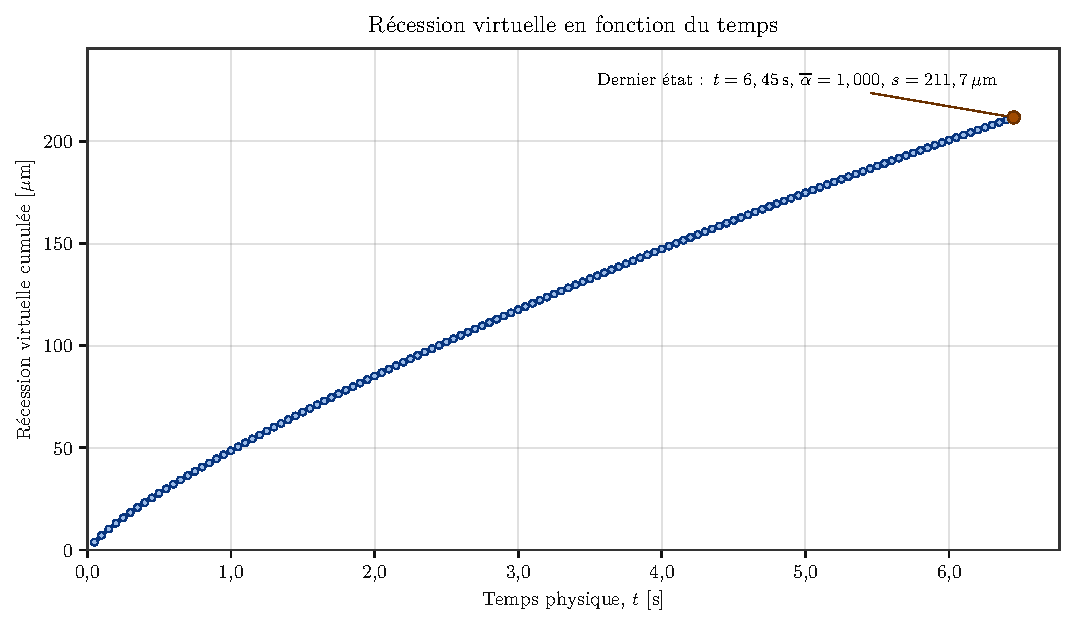
\includegraphics[width=0.96\textwidth]{../analysis/simulation2_recession_vs_time_fr.pdf}
\caption{Récession virtuelle cumulée en fonction du temps physique. La courbe
est mise à jour à partir des états entièrement synchronisés.}
\label{fig:sim2-recession-time}
\end{figure}

\begin{figure}[H]
\centering
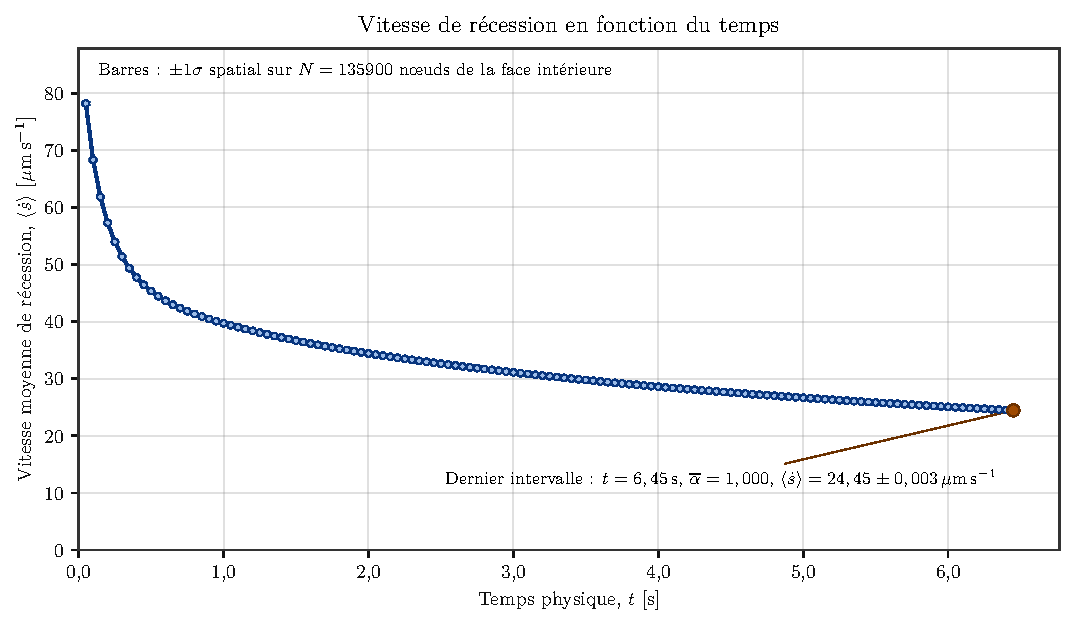
\includegraphics[width=0.96\textwidth]{../analysis/simulation2_recession_rate_vs_time_fr.pdf}
\caption{Vitesse moyenne de récession sur les 135\,900 noeuds de la surface
interne. Les barres représentent \(\pm1\sigma\) spatial.}
\label{fig:sim2-rate-time}
\end{figure}

\begin{figure}[H]
\centering
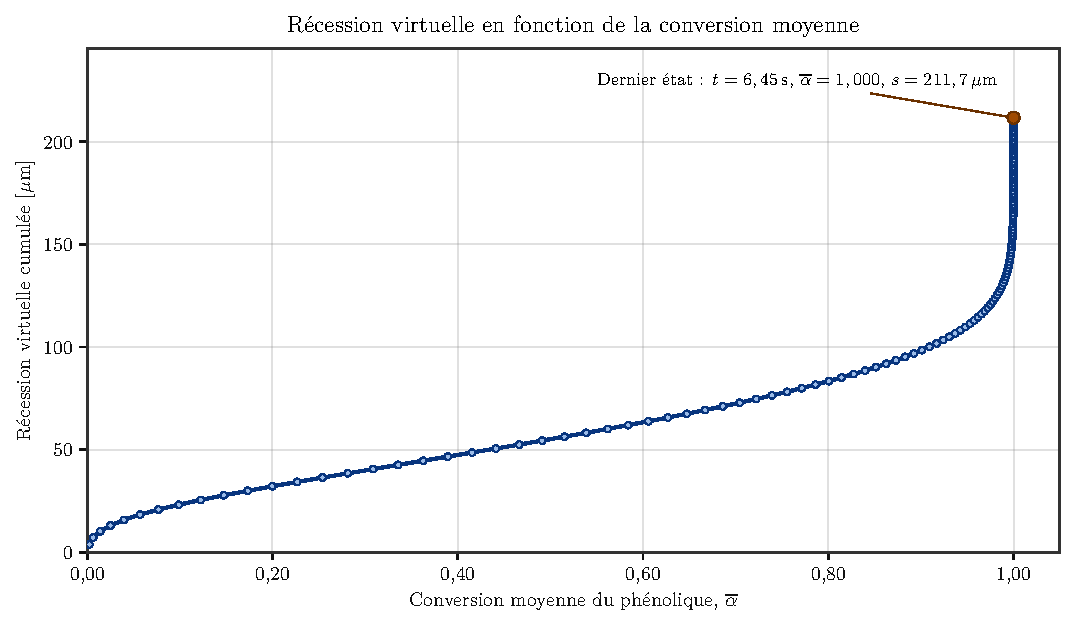
\includegraphics[width=0.96\textwidth]{../analysis/simulation2_recession_vs_alpha_avg_fr.pdf}
\caption{Récession virtuelle en fonction de la conversion moyenne. La courbe
montre que la récession continue après la quasi-saturation de \(\bar\alpha\).}
\label{fig:sim2-recession-alpha}
\end{figure}

\begin{figure}[H]
\centering
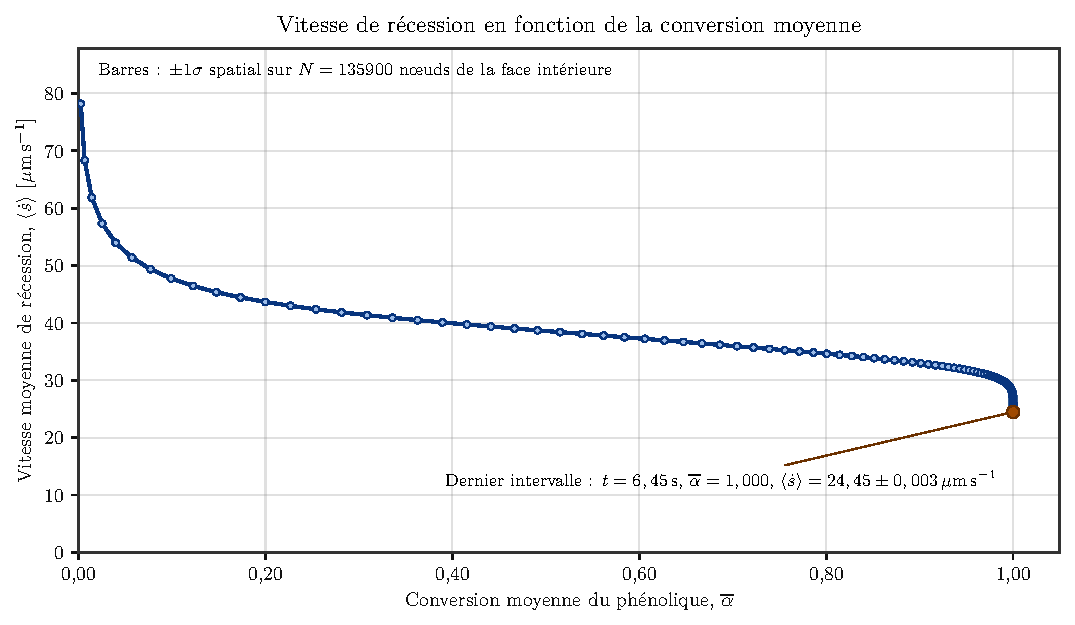
\includegraphics[width=0.96\textwidth]{../analysis/simulation2_recession_rate_vs_alpha_avg_fr.pdf}
\caption{Vitesse de récession en fonction de la conversion moyenne, avec
\(\pm1\sigma\) spatial.}
\label{fig:sim2-rate-alpha}
\end{figure}

\subsubsection{Profils spatiaux de conversion et de vitesse de pyrolyse}

Afin de permettre une comparaison directe avec la simulation 1, les mêmes
cinq familles de profils ont été reconstruites à partir des dix partitions
DMP de la simulation 2. Les états sauvegardés à
\(t=1,\ldots,6~\si{s}\) sont présents exactement; aucune interpolation
temporelle n'est donc employée. En revanche, le maillage radial ne fournit pas
un nœud dans chacun des cent rubans de 1\,\%. Les rubans sans observation sont
hachurés et seule l'enveloppe tracée y est interpolée linéairement. Cette
convention améliore la continuité visuelle sans créer de résolution physique
supplémentaire.

Les graphes radiaux montrent aussi la ligne verticale
\(d=s(t)\), où \(s(t)\) est la récession cumulée calculée par le bilan
énergétique du contrôleur. À ce stade, aucune bande n'a été supprimée : cette
ligne est donc une position de récession \emph{virtuelle} à l'intérieur de la
première couche encore maillée, et non une frontière géométrique déjà déplacée.
Elle ne doit pas être confondue avec un contour de conversion \(\alpha\).

\begin{figure}[H]
\centering
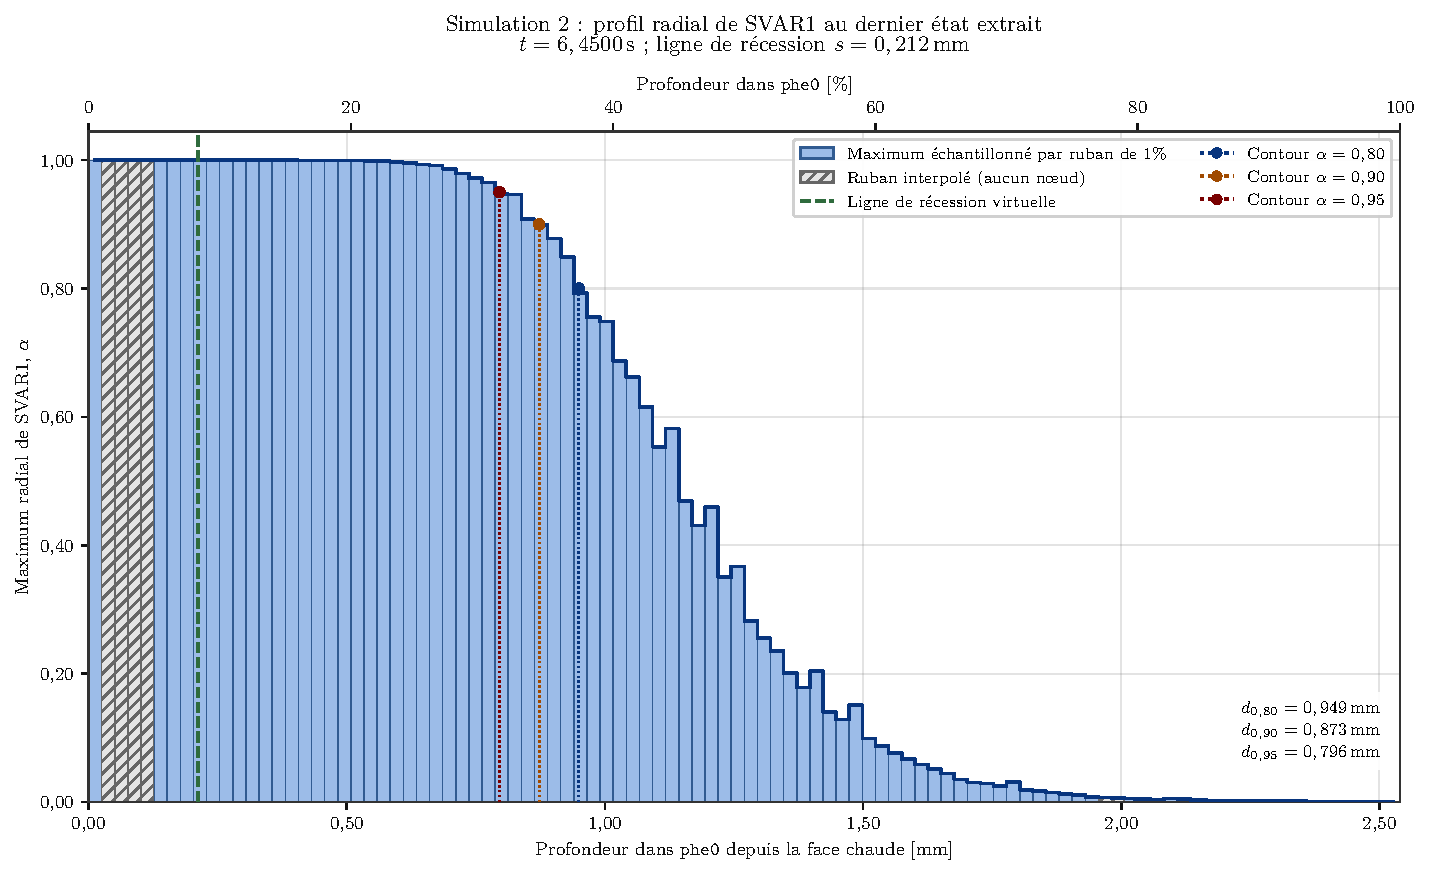
\includegraphics[width=0.98\textwidth]
{../analysis/simulation2_svar1_radial_profile_1pct_fr.pdf}
\caption{Profil radial du maximum de \code{SVAR1} au dernier état commun
extrait, avec les contours de conversion et la ligne de récession virtuelle.
Les rubans hachurés ne contiennent aucun nœud de résultat.}
\label{fig:sim2-svar1-radial-fr}
\end{figure}

\clearpage
\begin{figure}[H]
\centering
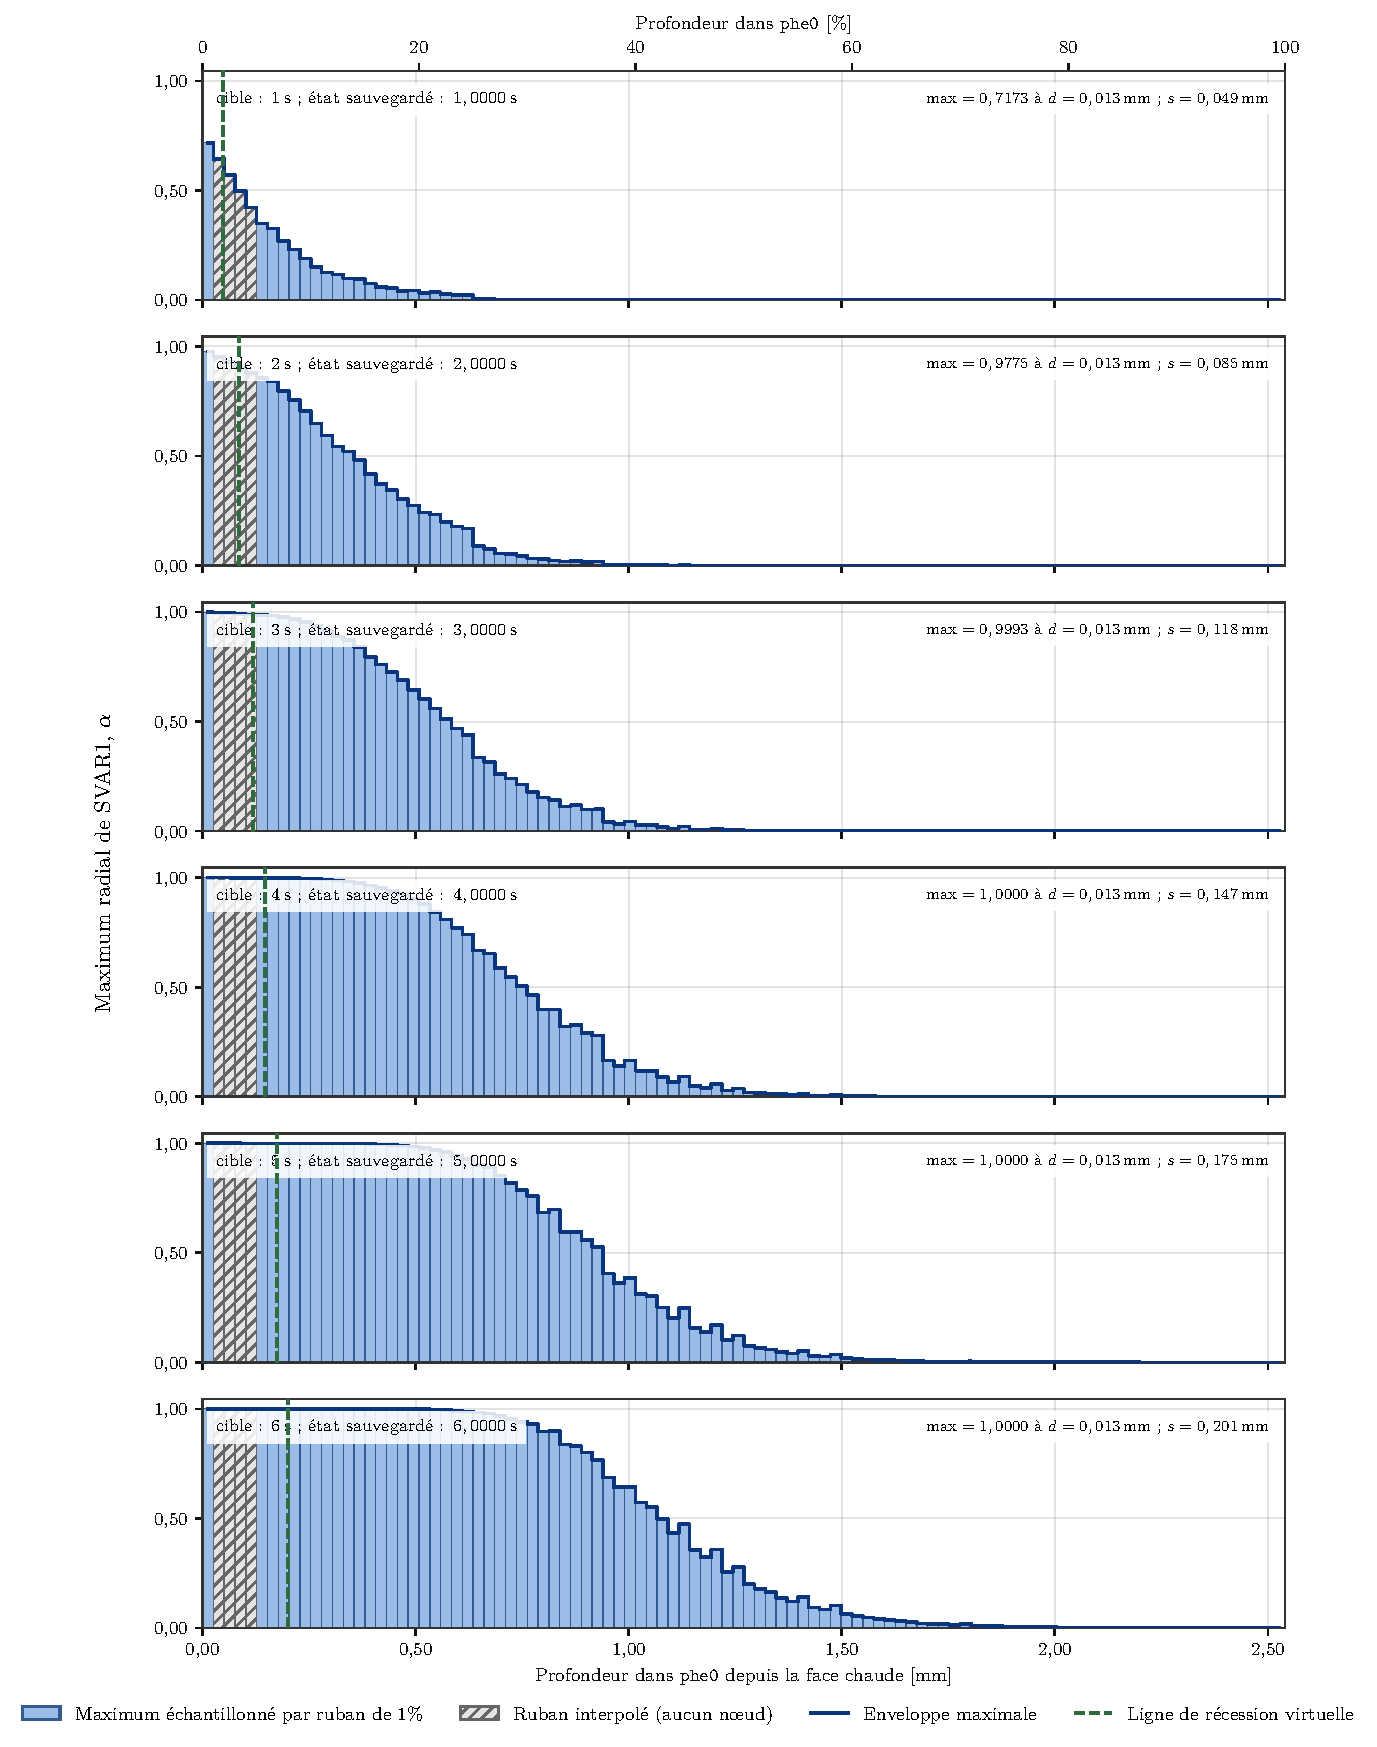
\includegraphics[height=0.80\textheight,width=0.96\textwidth,keepaspectratio]
{../analysis/simulation2_svar1_radial_time_profiles_1pct_fr.pdf}
\caption{Évolution du maximum radial de \code{SVAR1} dans la simulation 2.
La ligne verte discontinue indique, dans chaque panneau, la position cumulée
de la récession virtuelle.}
\label{fig:sim2-svar1-radial-time-fr}
\end{figure}

\clearpage
\begin{figure}[H]
\centering
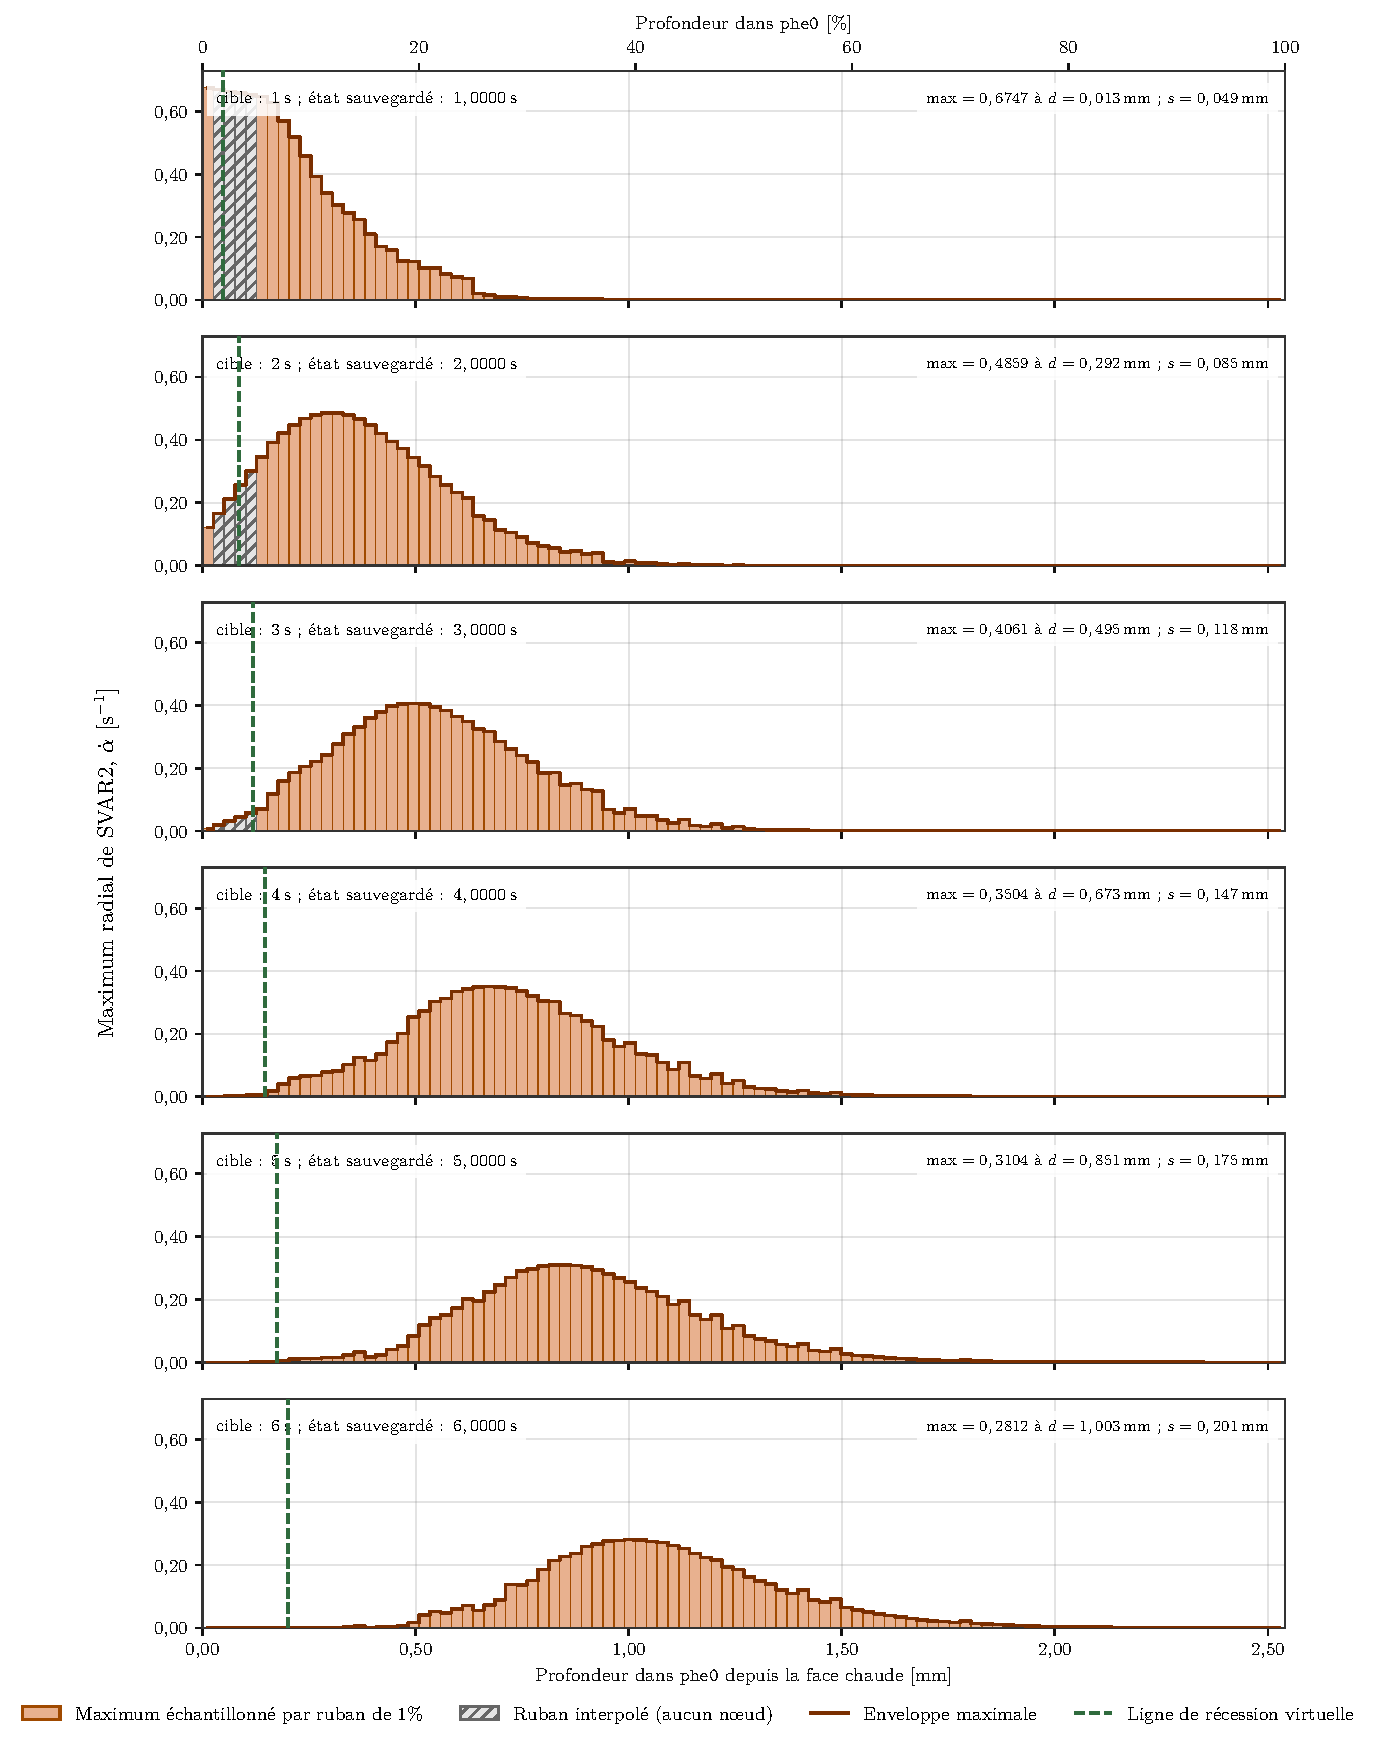
\includegraphics[height=0.80\textheight,width=0.96\textwidth,keepaspectratio]
{../analysis/simulation2_svar2_radial_time_profiles_1pct_fr.pdf}
\caption{Évolution du maximum radial de \code{SVAR2}. Le déplacement du
maximum de vitesse de pyrolyse et la progression de la ligne de récession
virtuelle sont représentés sur la même coordonnée radiale.}
\label{fig:sim2-svar2-radial-time-fr}
\end{figure}

\clearpage
\begin{figure}[H]
\centering
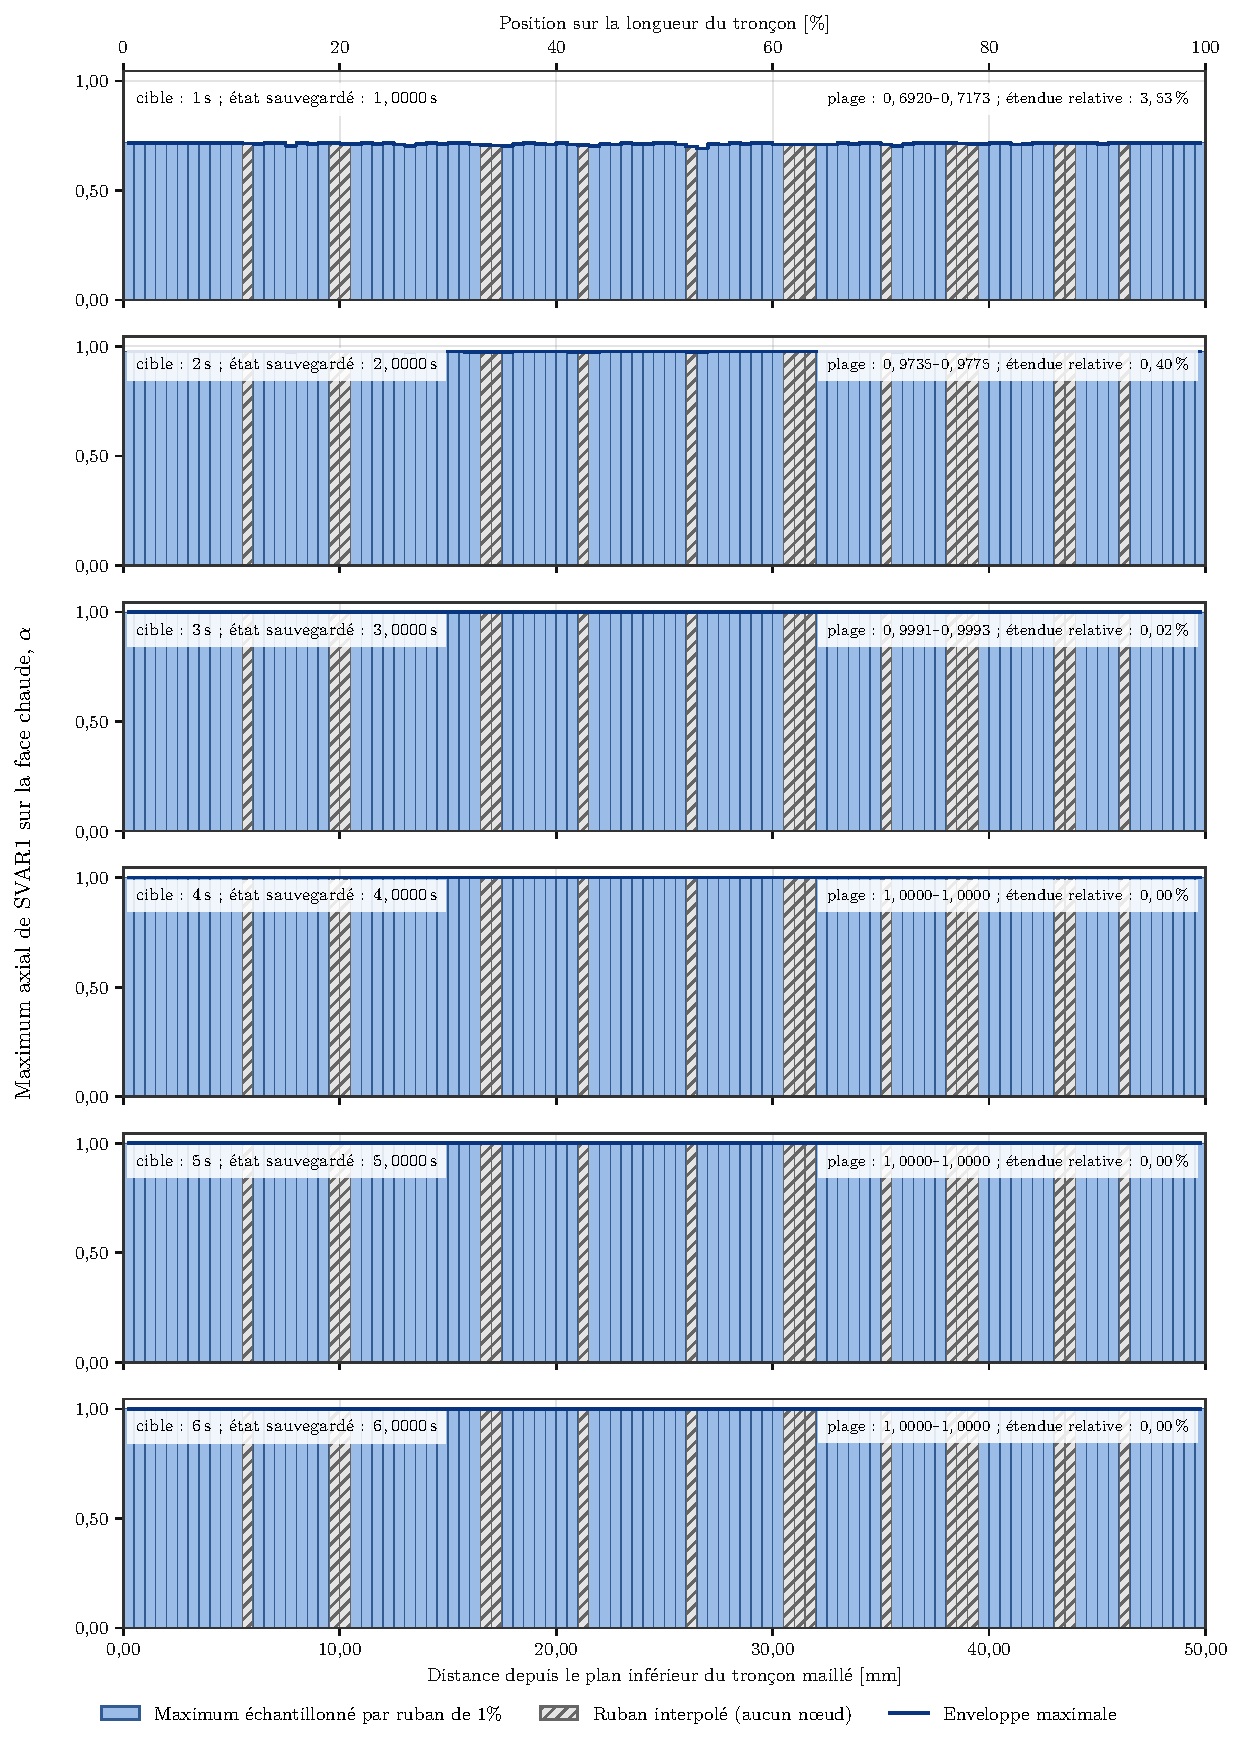
\includegraphics[height=0.80\textheight,width=0.96\textwidth,keepaspectratio]
{../analysis/simulation2_svar1_axial_time_profiles_1pct_fr.pdf}
\caption{Dépendance axiale de \code{SVAR1} sur la face intérieure chaude de la
simulation 2. L'axe axial ne porte pas de ligne de récession, car celle-ci est
définie suivant la coordonnée radiale.}
\label{fig:sim2-svar1-axial-time-fr}
\end{figure}

\clearpage
\begin{figure}[H]
\centering
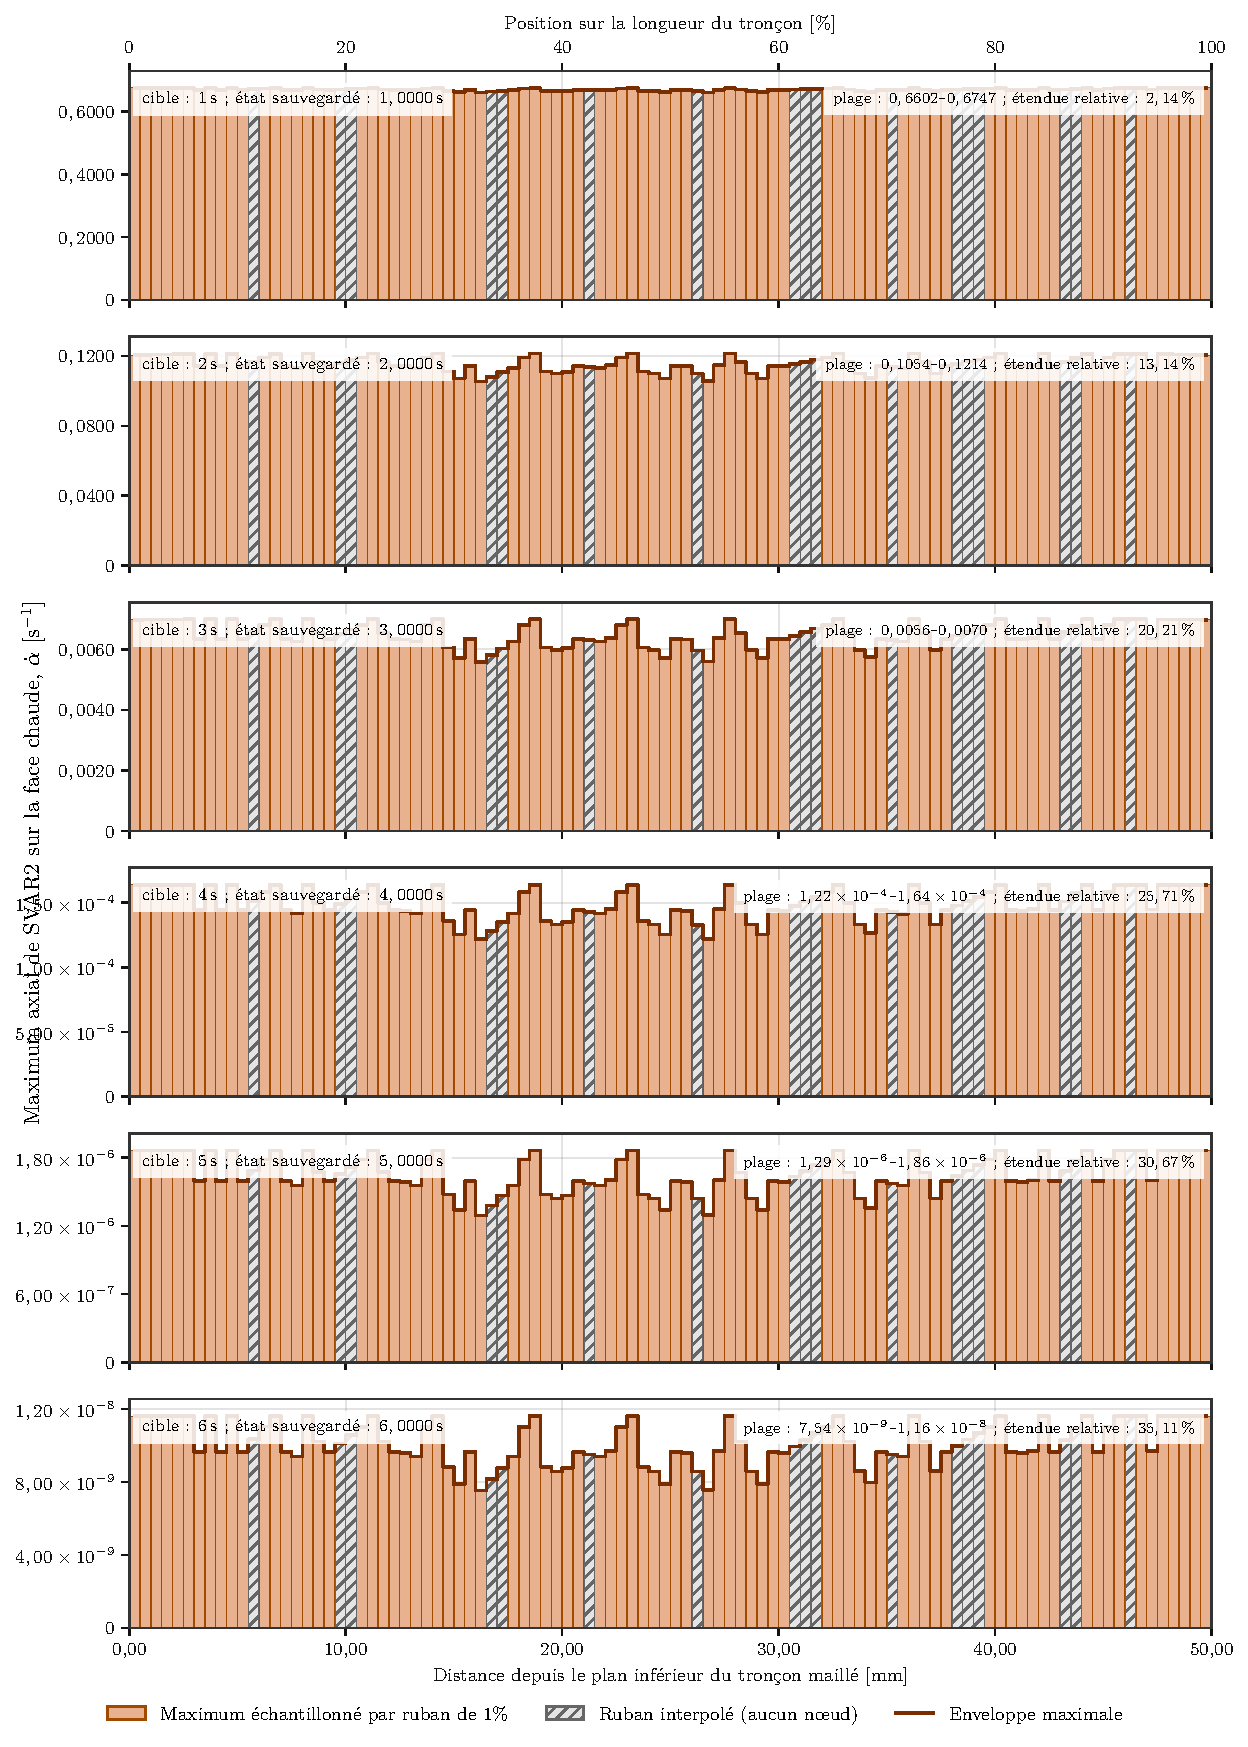
\includegraphics[height=0.80\textheight,width=0.96\textwidth,keepaspectratio]
{../analysis/simulation2_svar2_axial_time_profiles_1pct_fr.pdf}
\caption{Dépendance axiale de \code{SVAR2} sur la face intérieure chaude de la
simulation 2. Une échelle verticale propre à chaque panneau rend visibles les
faibles valeurs après saturation de la surface.}
\label{fig:sim2-svar2-axial-time-fr}
\end{figure}
\clearpage

Les données conservent 16 rubans radiaux et 17 rubans axiaux sans nœud,
exactement signalés par les hachures. À \SI{1}{s}, le maximum radial de
conversion vaut \(\alpha_\mathrm{max}=0{,}7173\); il atteint numériquement
l'unité à \SI{6}{s}. Le maximum de vitesse de pyrolyse diminue simultanément
de \SI{0.6747}{s^{-1}} à \SI{0.2812}{s^{-1}} et migre de
\SI{0.0127}{mm} à \SI{1.0033}{mm} de la face chaude. Au dernier état extrait,
\SI{6.15}{s}, il vaut \SI{0.2766}{s^{-1}} à
\SI{1.0287}{mm}.

La ligne de récession passe de \SI{0.0486}{mm} à \SI{1}{s} à
\SI{0.2006}{mm} à \SI{6}{s}, puis \SI{0.2044}{mm} à
\SI{6.15}{s}. À partir de \SI{2}{s}, elle demeure nettement en amont du
maximum de \code{SVAR2}. Les figures séparent ainsi visuellement deux
mécanismes différents : la zone volumique où la pyrolyse est la plus active et
la position cumulée de matière que le bilan énergétique permettrait de
récessionner. Sur la face chaude, \code{SVAR1} devient axialement uniforme à
l'unité; les variations relatives tardives de \code{SVAR2} atteignent environ
35\,\%, mais seulement sur des valeurs absolues de l'ordre de
\(10^{-8}~\si{s^{-1}}\), donc négligeables physiquement.

\clearpage
\begin{figure}[H]
\centering
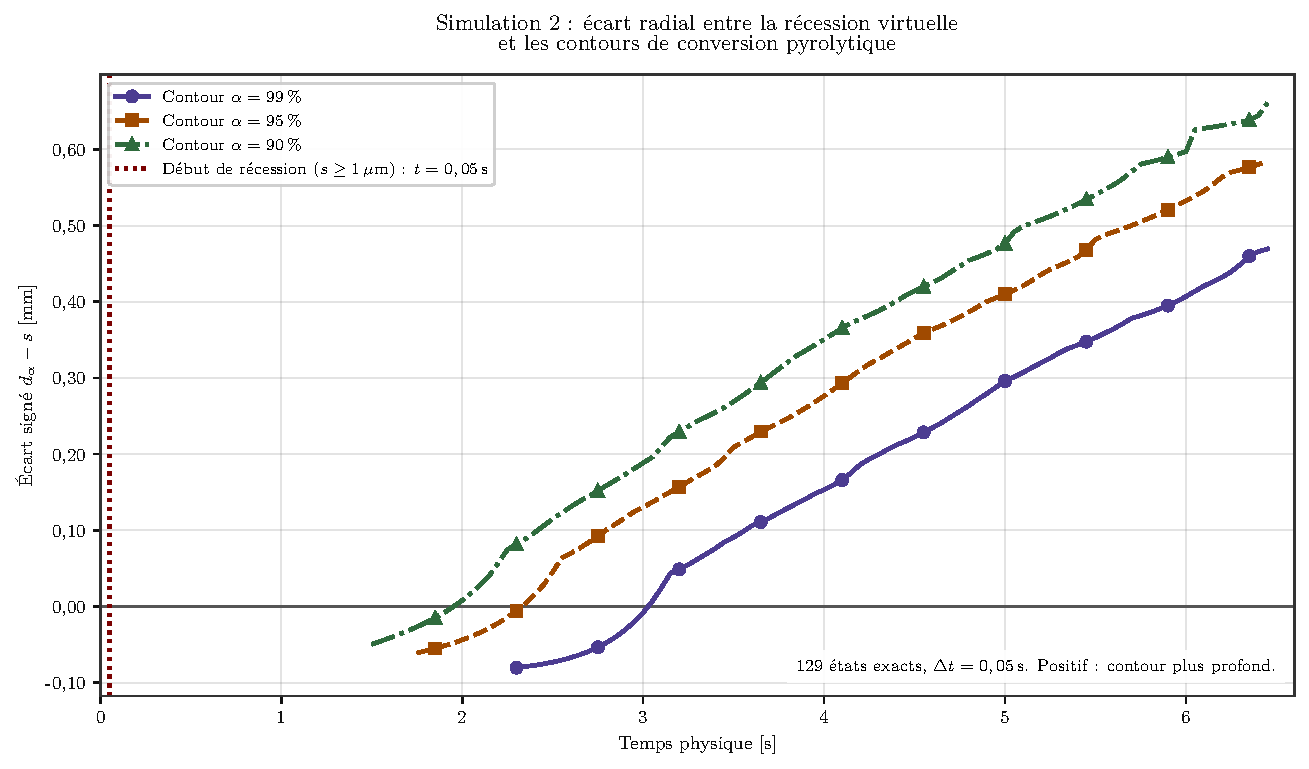
\includegraphics[width=0.94\textwidth]
{../analysis/simulation2_recession_to_pyrolysis_contours_vs_time_fr.pdf}
\caption{Écart radial signé entre la ligne de récession virtuelle et les
contours de conversion pyrolytique à 99\,\%, 95\,\% et 90\,\%.
L'écart est défini par \(\Delta d_\alpha=d_\alpha-s\) : une valeur positive
place le contour plus profondément dans la paroi que la récession. La ligne
verticale pointillée marque le premier état où la récession virtuelle atteint
\SI{1}{\micro m}.}
\label{fig:sim2-recession-contour-distance-fr}
\end{figure}

Les contours sont calculés par interpolation spatiale de l'enveloppe radiale
de \code{SVAR1} sur les 124 états synchronisés, espacés de
\SI{0.05}{s} entre \SI{0.05}{s} et \SI{6.20}{s}; aucune interpolation
temporelle n'est ajoutée. La ligne verticale à \SI{0.05}{s} indique le
premier état où \(s\geq\SI{1}{\micro m}\), avec
\(s=\SI{3.802}{\micro m}\). Ce seuil micrométrique évite d'assimiler un
résidu d'arrondi à l'apparition du front tout en restant très inférieur à la
résolution radiale du modèle. Une courbe ne commence que lorsque son seuil de
conversion est effectivement atteint : aucun zéro artificiel ne remplace les
données absentes. Les contours à 90\,\%, 95\,\% et 99\,\% apparaissent
respectivement à \SI{1.50}{s}, \SI{1.75}{s} et \SI{2.30}{s}, initialement en
amont de la récession, avec
\(\Delta d_\alpha=\SI{-0.0497}{mm}\), \SI{-0.0611}{mm} et
\SI{-0.0803}{mm}. Ils dépassent ensuite la ligne de récession à
\SI{2.00}{s}, \SI{2.35}{s} et \SI{3.05}{s}. Au dernier état extrait,
\SI{6.20}{s}, les séparations atteignent respectivement
\SI{0.4324}{mm}, \SI{0.5639}{mm} et \SI{0.6314}{mm} pour les contours à
99\,\%, 95\,\% et 90\,\%. La croissance de ces trois écarts montre que le
front de conversion progresse plus rapidement dans l'épaisseur que la
récession virtuelle.

\subsubsection{Interprétation provisoire et travaux restants}

Le résultat principal à ce stade est double. D'une part, la chaîne numérique
\code{UserMatTh} -- dégazage -- soufflage -- récession -- redémarrage distribué
fonctionne sur plus de cent macro-pas sans perte de continuité. D'autre part,
avec \(H_\mathrm{eff}=\SI{35}{MJ.kg^{-1}}\), la récession reste inférieure à une
bande à \SI{6.15}{s}; le pilote ne prédit donc encore aucun déplacement
discret de la frontière chaude.

La fin à \SI{7}{s} devra remplacer cet instantané par le bilan final et vérifier
si la première bande est franchie. Le rapport devra ensuite être complété par :
(i) les bilans massique et énergétique fermés; (ii) une comparaison PCG/SPARSE
incluant mémoire et temps mur; (iii) une étude de convergence avec 20 à 40
bandes radiales; (iv) des sensibilités à \(H_\mathrm{eff}\), \(h_0\), au pas de
temps et aux propriétés du char; et (v) la comparaison avec un essai
instrumenté. En l'absence de ces étapes, la récession calculée demeure un
indicateur de performance du modèle, pas une prédiction qualifiée du moteur.

% ============================================================================
\clearpage
\begin{thebibliography}{99}

\bibitem{ansys-usermatth}
ANSYS, Inc., \emph{UserMatTh --- User-Defined Thermal Material Model},
Mechanical APDL Programmer's Reference, version 2026 R1,
\url{https://ansyshelp.ansys.com/public/Views/Secured/corp/v261/en/ans_prog/Z7K4r1e5lcd.html},
consulté le 15 juillet 2026.

\bibitem{ansys-birthdeath}
ANSYS, Inc., \emph{Using Element Birth and Death}, Mechanical APDL Advanced
Analysis Guide,
\url{https://ansyshelp.ansys.com/public/Views/Secured/corp/v251/en/ans_adv/Hlp_G_ADV6_2.html},
consulté le 15 juillet 2026.

\bibitem{ansys-ekill}
ANSYS, Inc., \emph{EKILL --- Deactivates an element}, Mechanical APDL Command
Reference,
\url{https://ansyshelp.ansys.com/public/Views/Secured/corp/v242/en/ans_cmd/Hlp_C_EKILL.html},
consulté le 15 juillet 2026.

\bibitem{ewing2013}
M. E. Ewing, T. S. Laker et D. T. Walker, \emph{Numerical Modeling of
Ablation Heat Transfer}, NASA NTRS 20140008557, 2013,
\url{https://ntrs.nasa.gov/citations/20140008557}.

\bibitem{amar2010}
A. J. Amar, N. D. Calvert et B. S. Kirk, \emph{Development and Verification of
the Charring Ablating Thermal Protection Implicit System Solver}, NASA NTRS
20110000471, 2010,
\url{https://ntrs.nasa.gov/citations/20110000471}.

\bibitem{amar2016}
A. J. Amar, A. B. Oliver, B. S. Kirk, G. Salazar et J. Droba,
\emph{Overview of the CHarring Ablator Response (CHAR) Code}, NASA NTRS
20160005889, 2016,
\url{https://ntrs.nasa.gov/citations/20160005889}.

\bibitem{clark1972}
R. K. Clark, \emph{A Numerical Analysis of the Transient Response of an
Ablation System Including Effects of Thermal Nonequilibrium, Mass Transfer and
Chemical Kinetics}, NASA-TM-X-68853, NASA NTRS 19730002381, 1972,
\url{https://ntrs.nasa.gov/citations/19730002381}.

\bibitem{bessire2023}
B. K. Bessire, \emph{Analysis of Pyrolysis Products from Ablative TPS}, NASA
NTRS 20230000843, 2023,
\url{https://ntrs.nasa.gov/citations/20230000843}.

\bibitem{nasa-testing}
NASA Ames Research Center, \emph{Thermal Protection Materials Branch ---
Testing and Fabrication}, description des mesures TGA, DSC et LFA,
\url{https://www.nasa.gov/thermal-protection-materials-branch-testing-and-fabrication/},
consulté le 15 juillet 2026.

\bibitem{local-step}
MIT Rocket Team, \code{motoren.stp}, géométrie STEP AP214 du projet, fichier
local analysé le 15 juillet 2026.

\bibitem{local-model}
MIT Rocket Team, \code{EngineeringData.xml}, \code{ds.dat},
\code{phenolic_pyrolysis_native.apdl} et \code{usermatth.F}, artefacts locaux de
la simulation ANSYS Mechanical 2026 R1, état analysé le 15 juillet 2026.

\bibitem{local-results}
MIT Rocket Team, \code{file0.rth}--\code{file7.rth}, \code{file.nlh},
\code{file.mntr}, \code{solve.out} et
\code{svar1_radial_profile_1pct.csv}, sorties locales de la simulation ANSYS
Mechanical 2026 R1, dernier état convergé à \(t=\SI{6.38561694}{s}\), analysées
le 16 juillet 2026.

\end{thebibliography}

\clearpage
\listoffigures
\listoftables

\vfill
\section*{Déclaration d'Utilisation de l'IA}

L'IA a été utilisé pour générer une partie de ce document et pour une partie de la conception du contenu.
\end{document}
